\chapter{آموزش شبکه، Embedding بافتی و تبدیل نویسه به واج}

این فصل از سه بخش به‌هم‌پیوسته ساخته شده است. بخش نخست، مرور سریعی بر فرایند آموزش شبکه‌های عصبی است؛ مفاهیم پایه (انتشار رو‌به‌جلو، تابع خطا، پس‌انتشار و به‌روزرسانی وزن‌ها) در فصل پیش آمده بودند، بنابراین اینجا فقط به آنچه برای ادامه لازم است، یعنی طراحی لایهٔ خروجی، تفاوت آموزش و استنتاج، و پدیدهٔ بیش‌برازش، پرداخته می‌شود. بخش دوم، \eng{Embedding}های بافتی را بررسی می‌کند: از روش‌های ساخت آن‌ها و مدل \eng{BERT} تا تحلیل فضای \eng{Embedding} با قیاس برداری (\eng{Analogy}) و \term{کاوش}{Probing}. بخش سوم به هدف اصلی بازمی‌گردد: سامانهٔ تبدیل متن به گفتار (\eng{TTS}) باید برای هر واژه تلفظ درست را پیدا کند. در آنجا همین ابزارها برای رفع ابهام هم‌نویسه‌ها (\eng{Homograph}) و پیش‌بینی تلفظ واژه‌های ناشناخته (\eng{G2P}) به کار می‌روند.

\section{مرور فرایند آموزش شبکهٔ عصبی}

\subsection{چرخهٔ آموزش}
آموزش یک شبکه از مقداردهی تصادفی اولیهٔ وزن‌ها آغاز می‌شود و سپس چهار گام زیر برای هر دسته از داده‌ها تکرار می‌گردد (شکل~\ref{fig:ch09-train-loop}):
\begin{enumerate}
  \item \term{انتشار رو‌به‌جلو}{Feedforward}: ورودی با کمک وزن‌ها، بایاس‌ها و توابع فعال‌سازی از لایه‌ها عبور می‌کند.
  \item \textbf{خروجی}: لایهٔ آخر مقدار پیش‌بینی‌شده (امتیاز، احتمال یا مقدار عددی) را می‌دهد.
  \item \term{تابع خطا}{Loss}: خروجی با مقدار درست، یعنی \term{حقیقت مبنا}{Ground Truth}، مقایسه می‌شود و یک عدد برای «میزان خطا» به دست می‌آید.
  \item \term{پس‌انتشار و بهینه‌سازی}{Backpropagation}: با قاعدهٔ زنجیره‌ای، سهم هر وزن در خطا (گرادیان) حساب می‌شود و وزن‌ها در خلاف جهت گرادیان و به‌اندازهٔ نرخ یادگیری اصلاح می‌شوند.
\end{enumerate}
جزئیات ریاضی این گام‌ها (از جمله \mbox{$w_{\text{new}}=w_{\text{old}}-\eta\,\partial E/\partial w$} و مفهوم \eng{Loss Landscape}) در فصل قبل آمده است. استاد این نکته را تکرار کرد که تا وقتی خروجی تخمینی با واقعیت برابر نشده باشد، هنوز چیزی برای یادگرفتن وجود دارد.

\begin{figure}[htbp]
\centering
\begin{tikzpicture}[rtl, 
  box/.style={draw,rounded corners=2pt,minimum height=0.9cm,minimum width=2.3cm,align=center,fill=blue!6,font=\small},
  ar/.style={-{Stealth[length=2mm]},thick}]
  \node[box,fill=gray!15] (i) {مقداردهی\\تصادفی وزن‌ها};
  \node[box,right=0.7cm of i] (f) {\lr{Feedforward}\\خروجی};
  \node[box,right=0.7cm of f] (l) {\lr{Loss}\\مقایسه با واقعیت};
  \node[box,right=0.7cm of l] (b) {\lr{Backprop}\\گرادیان};
  \node[box,right=0.7cm of b] (u) {به‌روزرسانی\\وزن‌ها};
  \draw[ar] (i)--(f); \draw[ar] (f)--(l); \draw[ar] (l)--(b); \draw[ar] (b)--(u);
  \draw[ar,dashed] (u.south) -- ++(0,-0.7) -| node[pos=0.25,below,font=\small]{دستهٔ بعدی داده} (f.south);
\end{tikzpicture}
\caption{چرخهٔ آموزش شبکهٔ عصبی (شکل افزوده)}
\label{fig:ch09-train-loop}
\end{figure}

\subsection{طراحی لایهٔ خروجی بر اساس نوع مسئله}
نکتهٔ مورد تأکید استاد این بود که \emph{خروجی شبکه باید با \eng{Task} هم‌خوان طراحی شود}. سه حالت اصلی وجود دارد :

\boardfigure{0.8}{ch09-board-nn-img05.png}{انتخاب لایهٔ خروجی بر اساس نوع مسئله: رگرسیون با یک خروجی خطی، دسته‌بندی دودویی با یک خروجی سیگموید و دسته‌بندی چندکلاسه با سافت‌مکس.}

\begin{table}[htbp]
\centering
\small
\begin{tabular}{p{2.6cm}p{3.4cm}p{3.3cm}p{3.5cm}}
\toprule
\textbf{نوع مسئله} & \textbf{لایهٔ خروجی} & \textbf{تابع خطا} & \textbf{مثال از پردازش گفتار}\\
\midrule
\eng{Regression} & یک خروجی خطی (مقدار پیوسته) & \eng{MSE} & پیش‌بینی مقدار فرکانس پایه در یک لحظه\\
\eng{Binary Classification} & یک خروجی \eng{Sigmoid} و آستانه‌گذاری & \eng{Binary Cross-Entropy} & واکدار/بی‌واک، گفتار/سکوت، اسپم یا غیراسپم\\
\eng{Multi-class Classification} & \eng{Softmax} روی \eng{K} کلاس & \eng{Cross-Entropy} & تشخیص نوع احساس صدا، موضوع خبر، تلفظ درست یک واژه\\
\bottomrule
\end{tabular}
\caption{ارتباط نوع مسئله با لایهٔ خروجی و تابع خطا.}
\end{table}
\paragraph{رگرسیون.} فرض کنید بخش پیشین شبکه برداری مانند $X\in\mathbb{R}^{1\times 768}$ ساخته باشد. برای پیش‌بینی یک عدد (مثلاً $F_0$) کافی است یک لایهٔ خطی با $W\in\mathbb{R}^{768\times1}$ قرار دهیم:
\[
Y = XW + b,\qquad Y\in\mathbb{R}^{1\times1}.
\]
اگر مسئله پیچیده‌تر بود، می‌توان به‌جای یک لایه از ساختار \eng{Linear $\rightarrow$ Activation $\rightarrow$ Linear} (یک \eng{MLP}) استفاده کرد. استاد تأکید کرد که همیشه لازم نیست معماری پیچیده انتخاب شود؛ گاهی یک لایهٔ خطی ساده کافی است و پیچیده‌ترکردن باید بر اساس عملکرد مدل انجام شود.

\paragraph{دسته‌بندی دودویی.} خروجی یک \term{لاجیت}{Logit} است که از تابع سیگموید می‌گذرد و عددی در $(0,1)$ می‌دهد:
\[
\sigma(x)=\frac{1}{1+e^{-x}}.
\]
اگر خروجی $0.8$ باشد، مدل احتمال کلاس مثبت را ۸۰ درصد برآورد کرده است؛ با تعیین یک آستانه (\eng{Threshold}) کلاس نهایی مشخص می‌شود. روی تخته نوشته شده بود که سیگموید «برای هر خروجی احتمال مستقل می‌دهد و ترشولد می‌زنیم».

\paragraph{دسته‌بندی چندکلاسه.} برای تبدیل $K$ لاجیت \mbox{$z_1,\dots,z_K$} به یک توزیع احتمال از \eng{Softmax} استفاده می‌شود؛ این تابع «احتمال کلاس‌ها را با هم نرمال می‌کند تا مجموعشان ۱ شود»:
\[
P(y=i)=\frac{e^{z_i}}{\sum_{j=1}^{K}e^{z_j}},\qquad \sum_{i=1}^{K}P(y=i)=1 .
\]
در پیش‌بینی توکن بعدی، اگر واژگان $V$ توکن داشته باشد، لایهٔ خروجی بردار $1\times768$ را با ماتریس $768\times V$ ضرب می‌کند و یک بردار $1\times V$ از لاجیت‌ها به دست می‌آید؛ \eng{Softmax} به هر توکن یک احتمال می‌دهد.

\begin{addedbox}{سیگموید مستقل یا سافت‌مکس؟}
در دسته‌بندی چندکلاسهٔ معمولی هر نمونه دقیقاً یک برچسب دارد، پس کلاس‌ها باید با هم رقابت کنند و \eng{Softmax} مناسب است. اگر هر نمونه بتواند هم‌زمان چند برچسب داشته باشد (\eng{Multi-label})، برای هر برچسب یک سیگموید مستقل به کار می‌رود. این همان تفاوتی است که روی تخته با عبارت «احتمال مستقل» و «نرمال‌شده تا مجموع ۱» نشان داده شد.
\end{addedbox}

\subsection{تابع خطا و مثال پیش‌بینی توکن بعدی}
برای دسته‌بندی چندکلاسه با برچسب \eng{One-Hot}، تابع \eng{Cross-Entropy} به شکل زیر ساده می‌شود:
\[
L=-\sum_{k=1}^{K}y_k\log \hat y_k = -\log \hat y_{c},
\]
که در آن $c$ کلاس درست است؛ یعنی فقط احتمالی که مدل به پاسخ درست داده اهمیت دارد.

\boardfigure{0.7}{ch09-board-nn-img17.png}{مثال استاد: مدل برای واژهٔ «خواهم» احتمال $0.2$ را پیش‌بینی کرده و پاسخ درست ۱ است؛ برای «خوردم» و «بینم» پاسخ درست ۰ است.}

با احتمال $0.2$ برای پاسخ درست، خطا برابر \mbox{$-\log 0.2\approx 1.61$} است. اگر پس از چند گام اصلاح وزن‌ها، احتمال پاسخ درست به $0.9$ برسد، خطا به \mbox{$-\log 0.9\approx 0.105$} کاهش می‌یابد (لگاریتم طبیعی). پس شبکه یاد می‌گیرد به پاسخ درست احتمال بیشتری بدهد.

\begin{figure}[htbp]
  \centering
  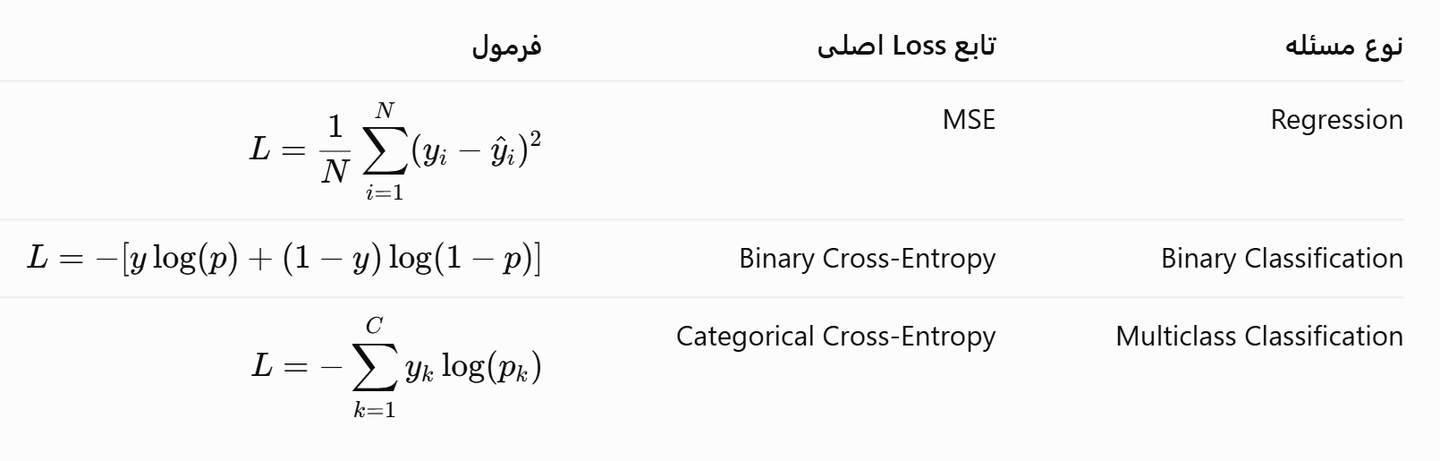
\includegraphics[width=0.85\textwidth]{../assets/figures/ch09-board-nn-img06.png}
  \caption{جدول انتخاب تابع خطا بر اساس نوع مسئله: \eng{MSE} برای رگرسیون، \eng{Binary Cross-Entropy} برای دسته‌بندی دودویی و \eng{Categorical Cross-Entropy} برای چندکلاسه \textit{(برگرفته از تختهٔ کلاس)}}
\end{figure}

\section{آموزش در برابر استنتاج}

در فاز \term{آموزش}{Training} پاسخ درست را داریم و می‌توانیم خطا را حساب کنیم؛ در فاز \term{استنتاج}{Inference} پاسخ درست در اختیار نیست و شبکه فقط یک توزیع احتمال تولید می‌کند. پرسش این است که از این توزیع چگونه خروجی نهایی را برداریم. استاد این تفاوت را روی تخته با عنوان «در فاز آموزش یک واقعیت داریم، بررسی می‌کنیم مدل به آن واقعیت چه مقداری داده» در برابر «در فاز اینفرنس» (\eng{Softmax}+\eng{Greedy}، یا \eng{Softmax}+\eng{Sampling}، یا \eng{Temperature}+\eng{Softmax}) نوشته بود.

\begin{table}[htbp]
\centering
\small
\begin{tabular}{p{3.0cm}p{5.4cm}p{5.6cm}}
\toprule
 & \textbf{آموزش} & \textbf{استنتاج}\\
\midrule
حقیقت مبنا & در دسترس است & در دسترس نیست\\
هدف & کمینه‌کردن خطا و اصلاح وزن‌ها & گرفتن خروجی از توزیع احتمال\\
وزن‌ها & در حال تغییرند & ثابت‌اند\\
\eng{Dropout} & فعال & غیرفعال\\
انتخاب خروجی & لازم نیست؛ خطا روی احتمال پاسخ درست حساب می‌شود & \eng{Greedy}، \eng{Sampling}، \eng{Top-k}، \eng{Top-p}، \eng{Temperature}\\
\bottomrule
\end{tabular}
\caption{مقایسهٔ آموزش و استنتاج (ردیف \eng{Dropout} افزوده شده است).}
\end{table}

\subsection{\eng{Greedy} و \eng{Sampling}}
\begin{itemize}
  \item \term{رمزگشایی حریصانه}{Greedy Decoding}: پراحتمال‌ترین گزینه انتخاب می‌شود، \mbox{$y=\arg\max_i P(y=i)$}. این روش قطعی است؛ برای توزیع \mbox{$(0.6,0.3,0.1)$} همیشه گزینهٔ اول برگزیده می‌شود.
  \item \term{نمونه‌گیری}{Sampling}: خروجی از روی توزیع احتمال نمونه‌برداری می‌شود، پس گزینه‌های کم‌احتمال‌تر هم شانس انتخاب دارند. این روش وقتی مفید است که تنوع خروجی مطلوب باشد (مثلاً تولید متن خلاقانه).
  \item \term{نمونه‌گیری \eng{Top-k}}{Top-k Sampling}: فقط $k$ گزینهٔ پراحتمال نگه داشته می‌شوند (مثلاً ۱۰ توکن برتر) و نمونه‌گیری از میان آن‌ها انجام می‌شود.
  \item \term{نمونه‌گیری \eng{Top-p}}{Nucleus Sampling}: توکن‌ها بر اساس احتمال مرتب می‌شوند و کوچک‌ترین مجموعه‌ای که مجموع احتمالش دست‌کم $p$ (مثلاً $0.9$) باشد نگه داشته می‌شود؛ نمونه‌گیری از همین مجموعه انجام می‌شود.
\end{itemize}
در کلاس به جست‌وجوی پرتویی (\eng{Beam Search}) نیز اشاره شد. این روش نمونه‌گیری نیست، بلکه به‌جای نگه‌داشتن فقط یک گزینه در هر گام، چند دنبالهٔ پراحتمال (پرتو) را هم‌زمان نگه می‌دارد و در پایان محتمل‌ترین دنباله را برمی‌گزیند.

\subsection{دما (\eng{Temperature})}
دما میزان «تیزی» توزیع احتمال را تنظیم می‌کند. لاجیت‌ها پیش از \eng{Softmax} بر $T$ تقسیم می‌شوند:
\[
P_i=\frac{e^{z_i/T}}{\sum_j e^{z_j/T}} .
\]
با $T=1$ همان \eng{Softmax} معمولی داریم؛ با $T\to0$ توزیع بسیار تیز می‌شود و به \eng{argmax} نزدیک می‌گردد؛ با $T$ بزرگ توزیع هموارتر می‌شود و در حد، به توزیع یکنواخت میل می‌کند. دمای بالا تنوع و تصادفی‌بودن را بیشتر می‌کند و در مقابل احتمال تولید خروجی نامناسب (مثلاً \eng{Hallucination}) هم بالاتر می‌رود؛ دمای پایین خروجی را تکرارپذیرتر می‌کند. دما لاجیت‌های یادگرفته‌شده را عوض نمی‌کند و فقط روش تبدیل آن‌ها به احتمال را هنگام تولید تغییر می‌دهد.

\begin{addedbox}{مثال عددی: اثر دما روی لاجیت‌ها}
فرض کنید لاجیت سه توکن \mbox{$z=(2.0,\;1.0,\;0.1)$} باشد. برای $T=1$ داریم \mbox{$e^{2}=7.389$}، \mbox{$e^{1}=2.718$} و \mbox{$e^{0.1}=1.105$}، مجموع $11.212$ و احتمال‌ها \mbox{$(0.66,\,0.24,\,0.10)$}. برای $T=0.2$ لاجیت‌ها ضرب در ۵ می‌شوند، یعنی \mbox{$(10,5,0.5)$}، و احتمال‌ها تقریباً \mbox{$(0.99,\,0.01,\,0.00)$} می‌شود؛ تقریباً \eng{Greedy}. برای $T=3$ لاجیت‌ها به \mbox{$(0.67,0.33,0.03)$} می‌رسند و احتمال‌ها \mbox{$(0.44,\,0.32,\,0.24)$} می‌شود؛ توزیع به یکنواخت نزدیک‌تر است.
\end{addedbox}

\coursefigure{0.62}{ch09-temperature.png}{اثر دما بر احتمال سه توکن فرضی با لاجیت‌های ثابت \mbox{$(2.0,1.0,0.1)$}: دمای کم توزیع را تیز و دمای زیاد آن را هموار می‌کند. (شکل افزوده)}

\begin{correctionbox}{\eng{Dropout} و استنتاج}
در کلاس \eng{Dropout} فقط به‌عنوان روشی برای کاهش وابستگی بیش‌ازحد به مسیرهای خاص شبکه معرفی شد. باید افزود که \eng{Dropout} تنها در زمان آموزش اعمال می‌شود؛ در استنتاج همهٔ نورون‌ها فعال‌اند (و مقیاس خروجی‌ها طوری تنظیم می‌شود که میانگین فعالیت تغییر نکند). این یکی از مثال‌هایی است که شبکه در آموزش و استنتاج دقیقاً یکسان رفتار نمی‌کند.
\end{correctionbox}

\section{تعمیم‌پذیری: کم‌برازش، بیش‌برازش و پیچیدگی مدل}

\subsection{داده‌های آموزش، اعتبارسنجی و آزمون}
برای فهمیدن اینکه مدل «به‌اندازهٔ کافی» آموزش دیده یا نه، تنها دیدن خطای داده‌های آموزشی کافی نیست؛ مدل باید روی داده‌ای ارزیابی شود که در به‌روزرسانی وزن‌ها به‌کار نرفته است. به همین دلیل مجموعه‌دادهٔ واحد را تقسیم می‌کنند (شکل~\ref{fig:ch09-split}): بخش \eng{Training} برای یادگیری وزن‌ها، بخش \eng{Validation} برای پایش آموزش و تصمیم‌هایی مانند توقف یا انتخاب ابرپارامتر، و بخش \eng{Test} برای گزارش نهایی. استاد روی تخته نوشت: «ارزیابی با داده‌هایی که در آموزش وزن‌ها استفاده نشده‌اند».

\begin{figure}[htbp]
  \centering
  \fbox{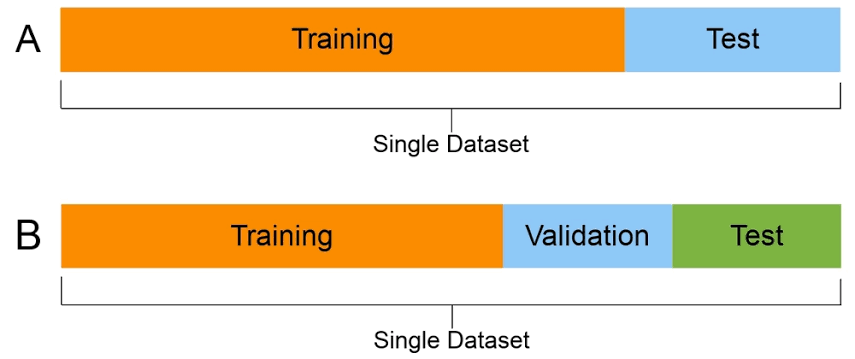
\includegraphics[width=0.65\textwidth]{../assets/figures/ch09-board-nn-img02.png}}
  \caption{تقسیم یک مجموعه‌داده: (الف) آموزش و آزمون؛ (ب) آموزش، اعتبارسنجی و آزمون. روی تخته به مجموعه‌دادهٔ \eng{LJ Speech} به‌عنوان نمونه‌ای از «یک مجموعه‌دادهٔ واحد» ارجاع داده شده بود. \textit{(برگرفته از تختهٔ کلاس)}}
  \label{fig:ch09-split}
\end{figure}

\begin{addedbox}{نکات تقسیم داده در گفتار}
\eng{LJ Speech} مجموعه‌ای تک‌گوینده با حدود $13\,100$ گفتار کوتاه و نزدیک به ۲۴ ساعت صداست. اگر به‌جای تقسیم تصادفی گفتارها، گفتارهای یک گوینده یا یک جملهٔ تکراری هم در آموزش و هم در آزمون بیایند، خطای آزمون خوش‌بینانه می‌شود؛ در کارهای چندگوینده معمولاً تقسیم بر اساس گوینده انجام می‌شود. مجموعهٔ آزمون نباید برای تنظیم مدل به‌کار برود.
\end{addedbox}

\subsection{سه وضعیت پس از آموزش}
\begin{itemize}
  \item \term{کم‌برازش}{Underfitting}: مدل حتی داده‌های آموزشی را هم خوب یاد نگرفته است (روی تخته: «مدل حتی داده‌های آموزشی را هم خوب یاد نگرفته است»).
  \item \term{برازش مناسب}{Good Fit}: الگوهای اصلی مسئله آموخته شده و عملکرد روی داده‌های تازه هم خوب است.
  \item \term{بیش‌برازش}{Overfitting}: مدل علاوه بر الگوی اصلی، جزئیات نامربوط و نویز داده آموزشی را هم حفظ کرده است («مدل داده‌های آموزشی را خوب یاد گرفته، اما تعمیم نمی‌دهد»).
\end{itemize}

\boardfigure{0.8}{ch09-board-nn-img24.png}{سه وضعیت برازش روی یک مجموعه نقطه: خط ساده (کم‌برازش)، منحنی هموار (متعادل) و منحنی بسیار نوسانی که از همهٔ نقاط می‌گذرد (بیش‌برازش).}

\begin{exambox}{مثال استاد از بیش‌برازش در گفتار}
فرض کنید در داده‌های آموزشی یک دستیار صوتی، هر بار که عبارت خاصی گفته شده، صدای فن هم در پس‌زمینه بوده است. مدل ممکن است به‌جای یادگیری الگوی گفتاری، صدای فن را نشانهٔ آن عبارت بگیرد. چنین مدلی روی داده آموزشی خوب عمل می‌کند، اما روی نمونه‌ای که همان عبارت را بدون صدای فن دارد اشتباه می‌کند.
\end{exambox}

\subsection{منحنی خطای آموزش و اعتبارسنجی}
با افزایش \eng{Epoch}، خطای آموزش معمولاً کم می‌شود. خطای اعتبارسنجی نخست کم می‌شود، اما از جایی به بعد ممکن است دوباره بالا برود. همان نقطهٔ کمینه بهترین توازن است، و افزایش خطای اعتبارسنجی همراه با کاهش خطای آموزش نشانهٔ بیش‌برازش است. توقف آموزش در این نقطه \term{توقف زودهنگام}{Early Stopping} نام دارد.

\boardfigure{0.6}{ch09-board-nn-img22.png}{نمودار خطای آموزش (آبی) و اعتبارسنجی (نارنجی) بر حسب \eng{Epoch}؛ خط‌چین عمودی محل توقف زودهنگام است. روی تخته زیر محور افقی «\eng{model complexity}: تعداد پارامترهای بیشتر $\leftrightarrow$ کمتر جنرال» هم نوشته شده بود.}

\coursefigure{0.95}{ch09-loss-curves.png}{سه رفتار نوعی در طول آموزش (سه نمودار اول) و رابطهٔ خطا با پیچیدگی مدل (نمودار آخر). مقادیر شبیه‌سازی‌شده‌اند و فقط برای نمایش مفهوم‌اند. (شکل افزوده)}

\subsection{\eng{Bias} و \eng{Variance}}
دو منبع اصلی خطا در یک مدل، «بایاس» و «واریانس» هستند (نباید بایاس به‌معنای خطا در این بحث را با پارامتر \eng{b} در $Wx+b$ اشتباه گرفت).

\begin{table}[htbp]
\centering
\small
\begin{tabular}{p{2.8cm}p{5.6cm}p{5.8cm}}
\toprule
 & \textbf{\eng{High Bias} (کم‌برازش)} & \textbf{\eng{High Variance} (بیش‌برازش)}\\
\midrule
نشانه & خطای آموزش و اعتبارسنجی هر دو زیاد و نزدیک به هم & خطای آموزش کم، خطای اعتبارسنجی بسیار بیشتر\\
تصویر شهودی & پیش‌بینی‌ها به هم نزدیک‌اند اما از جواب واقعی دورند & پیش‌بینی‌ها پراکنده‌اند؛ مدل با تغییر داده‌ها تغییر می‌کند\\
راهکار & مدل را پیچیده‌تر کن: لایه و نورون بیشتر، یا معماری مناسب‌تر & داده با کیفیت بیشتر، بررسی ناسازگاری‌های برچسب‌گذاری، متعادل‌کردن داده، \eng{Data Augmentation}، \eng{Regularization} (مثل \eng{Dropout} یا جریمهٔ وزن‌های بزرگ)\\
\bottomrule
\end{tabular}
\caption{مقایسهٔ بایاس بالا و واریانس بالا بر اساس یادداشت‌های تخته و کلاس.}
\end{table}

\begin{figure}[htbp]
  \centering
  \fbox{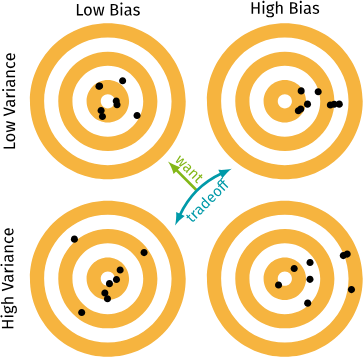
\includegraphics[width=0.38\textwidth]{../assets/figures/ch09-board-nn-img23.png}}
  \caption{مثال هدف‌گیری برای چهار ترکیب بایاس و واریانس؛ هدف مطلوب، بایاس و واریانس هر دو پایین است و در عمل میان آن دو مصالحه (\eng{Tradeoff}) وجود دارد. \textit{(برگرفته از تختهٔ کلاس)}}
\end{figure}

\begin{exambox}{از کجا بفهمیم تا کجا مدل را پیچیده‌تر کنیم؟}
پرسش تخته‌ای استاد این بود: «تا کجا به آموزش و پیچیده‌ترکردن مدل ادامه دهیم؟» پاسخ: تا جایی که خطای اعتبارسنجی بهتر می‌شود. معماری را باید بر پایهٔ عملکرد مدل تغییر داد، نه صرفاً با افزودن لایه و نورون. برای تشخیص مشکل، خطای آموزش به‌تنهایی کافی نیست و باید خطای اعتبارسنجی و وضعیت بایاس/واریانس هم بررسی شود.
\end{exambox}

\subsection{\eng{Regularization}}
\term{منظم‌سازی}{Regularization} هر روشی است که پیچیدگی مؤثر مدل را محدود می‌کند تا تعمیم بهتر شود.
\begin{itemize}
  \item \eng{Dropout}: در هر گام آموزش، خروجی تعدادی از نورون‌ها به‌طور تصادفی صفر می‌شود. شبکه مجبور می‌شود به مسیر یا ویژگی خاصی بیش‌ازحد تکیه نکند و وابستگی‌های بیش‌ازحد شکل‌گرفته بشکند.
  \item منظم‌سازی \eng{L1} و \eng{L2}: جمله‌ای به تابع خطا افزوده می‌شود که وزن‌های بزرگ را جریمه کند:
  \[
  L_{\text{total}}=L_{\text{task}}+\lambda\sum_i |w_i|\quad(\text{\lr{L1}}),\qquad
  L_{\text{total}}=L_{\text{task}}+\lambda\sum_i w_i^2\quad(\text{\lr{L2}}),
  \]
  که $\lambda$ شدت منظم‌سازی را تعیین می‌کند.
\end{itemize}

\begin{exambox}{پرسش: اگر وزن بزرگ برای یک ویژگی واقعاً خوب باشد چه؟}
روی تخته پرسیده شده بود: «اگر وزن بزرگ برای فیچر خوب و واقعی باشد چه؟» پاسخ استاد: منظم‌سازی بین وزن مفید و نامفید تمایز مستقیمی نمی‌گذارد و به‌طور کلی اعمال می‌شود. در یک شبکهٔ عمیق اطلاعات معمولاً با ترکیب تعداد زیادی ویژگی نمایش داده می‌شود و با وجود این محدودیت شبکه می‌تواند عملکرد خوبی حفظ کند. اگر وزن بزرگی برای کاهش خطای اصلی واقعاً لازم باشد، میان کاهش خطا و جریمهٔ وزن یک مصالحه شکل می‌گیرد و مدل آن وزن را کاملاً حذف نمی‌کند. بنابراین تضمینی نیست که هیچ ویژگی مفیدی آسیب نبیند؛ شدت $\lambda$ باید با توجه به عملکرد واقعی روی داده اعتبارسنجی انتخاب شود. در این بحث به اهمیت هم‌مقیاس‌کردن (\eng{Scaling}) ویژگی‌ها هم اشاره شد، چون جریمهٔ وزن به مقیاس ورودی‌ها حساس است.
\end{exambox}

\section{\eng{Embedding} ایستا و پویا (بافتی)}

\subsection{مرور}
\eng{Embedding} روشی برای نمایش واژه‌ها یا توکن‌ها به‌صورت بردارهای عددی چگال است (در برابر بردار تُنُک و دومقداری \eng{One-Hot}). روی تخته پرسش «ورودی چگونه نمایش داده می‌شود؟» مطرح بود و لایهٔ \eng{Embedding} به دو شاخه تقسیم می‌شد: ایستا (\eng{Static}) و پویا یا بافتی (\eng{Contextual}).

\begin{figure}[htbp]
\centering
\resizebox{\textwidth}{!}{%
\begin{tikzpicture}[rtl, 
  every node/.style={font=\small},
  dia/.style={diamond,aspect=2,draw=mainblue,thick,fill=softgreen,align=center,inner sep=2pt},
  bx/.style={draw=mainblue,thick,rounded corners=5pt,fill=softgreen,align=center,text width=6.9cm,inner sep=6pt},
  el/.style={draw=mainblue,thick,rounded corners=5pt,fill=softyellow,align=center,text width=6.9cm,inner sep=6pt},
  ar/.style={-{Stealth[length=2.5mm]},thick,mainblue}]
  \node[dia] (emb) at (0,0) {لایهٔ\\امبدینگ};
  \node[bx] (stat) at (-3.9,-3.8) {\textbf{امبدینگ ایستا} \lr{(Static)}\\[2pt]
    هر روشی که بردار خروجی یک کلمه تابعی از تمام جمله‌هایی باشد که در زمان آموزش، آن کلمه در بافت آن‌ها ظاهر شده است.\\[3pt]
    \textbf{در زمان استفاده:} کلمه تنها و بدون دیدن جمله وارد یک جدول \lr{(Lookup Table)} می‌شود.\\[3pt]
    \textbf{آنچه دانلود می‌کنیم:} فایلی که برای مثال برای «شیر» یک سطر با ۳۰۰ عدد دارد؛ بردار همیشه ثابت است و مستقیم از حافظه خوانده می‌شود.};
  \node[bx] (ctx) at (3.9,-3.8) {\textbf{امبدینگ پویا} \lr{(Dynamic / Contextual)}\\[2pt]
    هر روشی که بردار خروجی یک کلمه تابعی از کل کلمات موجود در جملهٔ فعلی باشد.\\[3pt]
    \textbf{در زمان استفاده:} کلمه در بستر کل جمله وارد شبکه می‌شود؛ شبکه کل جمله را پردازش می‌کند و بر اساس رابطهٔ کلمه با همسایه‌هایش بردار نهایی را می‌سازد.\\[3pt]
    \textbf{آنچه دانلود می‌کنیم:} وزن‌های شبکه \lr{(Weights \& Biases)}؛ بردار کلمه تا ورود جمله به شبکه وجود خارجی ندارد.};
  \node[el] (sa) at (-3.9,-9.6) {\textbf{\lr{Self-Attention}}\\ نمایش تمام موقعیت‌های ورودی را در اختیار داشته باش؛ ارتباط هر موقعیت را با موقعیت‌های دیگر محاسبه کن؛ بر اساس وزن‌های ارتباط، اطلاعات موقعیت‌ها را ترکیب کن تا نمایش جدید هر موقعیت به دست آید.};
  \node[el] (lstm) at (3.9,-9.6) {\textbf{\lr{LSTM}}\\ ورودی‌ها را به‌ترتیب پردازش کن؛ اطلاعات هر گام را از طریق حالت بازگشتی به گام بعد منتقل کن.};
  \draw[ar] (emb.south west) -- (stat.north);
  \draw[ar] (emb.south east) -- (ctx.north);
  \draw[ar] (ctx.south) -- (sa.north);
  \draw[ar] (ctx.south) -- (lstm.north);
\end{tikzpicture}}
\caption{دو شاخهٔ لایهٔ \eng{Embedding}: ایستا (جدول جست‌وجو) و پویا/بافتی (تابعی از کل جملهٔ فعلی)؛ دو بیضی پایین دو راه ساخت بافتی را نشان می‌دهند: \eng{Self-Attention} و پردازش ترتیبی با \eng{LSTM}. (بازسازی‌شده از تختهٔ کلاس)}
\end{figure}

\subsection{\eng{Embedding} ایستا}
در تعریف تخته‌ای: «هر روشی که طی آن بردار خروجی یک کلمه تابعی از تمامی جمله‌هایی باشد که در زمان آموزش، آن کلمه در بافت آن‌ها ظاهر شده است». مثال مهم \eng{Word2Vec} است (با دو روش آموزش \eng{CBOW} و \eng{Skip-gram} که در فصل قبل بررسی شد): ابتدا بردارها مقدار اولیه می‌گیرند، سپس با یک \eng{Task} آموزشی (پیش‌بینی واژهٔ هدف از بافت، یا بافت از واژهٔ هدف) تنظیم می‌شوند، و پس از پایان آموزش بخش پیش‌بینی کنار گذاشته می‌شود و فقط بردارها نگه داشته می‌شوند.

\textbf{در زمان استفاده}: واژه تنها و بدون دیدن جمله وارد یک \term{جدول جست‌وجو}{Lookup Table} می‌شود. آنچه دانلود می‌کنیم یک فایل است که مثلاً برای «شیر» یک سطر با ۳۰۰ عدد دارد و فرقی نمی‌کند منظور «شیر جنگل»، «شیر آب» یا «شیر خوراکی» باشد؛ بردار همیشه ثابت است و بدون نیاز به شبکهٔ عصبی مستقیماً از حافظه خوانده می‌شود. استاد این را با جمله‌ای دربارهٔ \eng{Word2Vec} جمع‌بندی کرد: مدل در زمان آموزش مبتنی بر بافت است (\eng{Context-based}) و در زمان استنتاج مستقل از بافت (\eng{Context-independent}).

\subsection{\eng{Embedding} پویا (بافتی)}
تعریف تخته‌ای: «هر روشی که طی آن بردار خروجی یک کلمه، تابعی از کل کلمات موجود در جملهٔ فعلی باشد». در زمان استفاده کل جمله وارد شبکه می‌شود، شبکه آن را پردازش می‌کند و بر اساس رابطهٔ واژه با همسایه‌هایش بردار نهایی را می‌سازد. در نتیجه:
\[
\text{ایستا: } E(w)=v_w,\qquad \text{بافتی: } E(w,C)=v_{w,C},\qquad E(\text{شیر},C_1)\neq E(\text{شیر},C_2).
\]
چیزی که دانلود می‌کنیم وزن‌ها و بایاس‌های شبکه است، و بردار یک واژه تا زمانی که جمله وارد شبکه نشود وجود خارجی ندارد. این تفاوت عملی مهمی دارد: بردار ایستا را می‌توان جدا ذخیره و مستقل استفاده کرد، ولی برای تولید بردار بافتی باید خود مدل (با همهٔ پارامترهایش) اجرا شود.

\begin{table}[htbp]
\centering
\small
\begin{tabular}{p{3.0cm}p{5.5cm}p{5.5cm}}
\toprule
 & \textbf{ایستا (\eng{Static})} & \textbf{پویا (\eng{Contextual})}\\
\midrule
بردار هر واژه & ثابت، یک بردار برای هر واژه & وابسته به جمله؛ هر رخداد بردار خودش را دارد\\
زمان استفاده & جست‌وجو در جدول (بدون شبکه) & اجرای شبکه روی کل جمله\\
خروجی دانلودی & فایل جدول بردارها & وزن‌های شبکه\\
نمونه & \eng{Word2Vec} (\eng{CBOW}، \eng{Skip-gram})، \eng{GloVe} & \eng{ELMo}، \eng{BERT}\\
\bottomrule
\end{tabular}
\caption{مقایسهٔ \eng{Embedding} ایستا و بافتی.}
\end{table}

\begin{correctionbox}{«شیر» در اینجا دو مسئلهٔ متفاوت را نشان می‌دهد}
واژهٔ «شیر» برای سه معنای جنگل، خوراکی و شیرآب هر سه یک‌جور تلفظ می‌شود (\lr{/ʃiːr/}). بنابراین مثال خوبی برای \emph{چندمعنایی} و محدودیت \eng{Embedding} ایستا است، اما یک \eng{Homograph} به‌معنای «هم‌نویسهٔ با تلفظ متفاوت» نیست. هم‌نویسه‌های واقعی از نوع مورد نیاز برای \eng{TTS} واژه‌هایی مانند «مَرد/مُرد» یا «کِرم/کَرَم» هستند که تلفظ‌شان فرق می‌کند. به همین دلیل در بخش مربوط به \eng{TTS} از «کرم»، «مرد» و «گرم» استفاده می‌کنیم.
\end{correctionbox}

\subsection{کاربرد \eng{Embedding} بافتی فراتر از رفع ابهام معنایی}
استاد تأکید کرد که \eng{Embedding} بافتی فقط برای واژه‌های چندمعنایی نیست. مثلاً در \term{تشخیص مرجع ضمیر}{Coreference Resolution}، در جمله‌ای مثل «من این کتاب را به علی دادم. او …» مدل باید ارتباط «او» را با «علی» (و نه «من» یا «کتاب») بتواند تشخیص دهد؛ یعنی بردارها باید تا حدی اطلاعات ارجاعی را هم در خود داشته باشند.

همچنین می‌توان از لایه‌های مختلف شبکه اطلاعات مختلفی بیرون کشید، مانند اطلاعات دستوری و برچسب نقش دستوری (\eng{POS})، ویژگی‌های معنایی، روابط وابسته به متن و حتی اطلاعات مرتبط با تلفظ. اینکه کدام اطلاعات در کدام لایه هست به معماری، داده و هدف آموزش بستگی دارد؛ برای بررسی آن از \eng{Probing} استفاده می‌کنیم (بخش~\ref{sec:ch09-probing}).

\section{راه‌های ساخت \eng{Embedding} بافتی}

مسئلهٔ اصلی این است: \emph{چگونه بردار یک واژه را وابسته به متن پیرامونش بسازیم؟} استاد تأکید کرد که نباید \eng{Contextual Embedding} را با معماری \eng{Transformer} یکی دانست؛ ابتدا باید مسئله را فهمید و بعد سراغ معماری خاصی رفت. دو رویکرد مطرح شد که روی تخته هم دو بیضی جدا برایشان کشیده شده بود.

\subsection{نگاه موازی: \eng{Self-Attention}}
مراحل روی تخته چنین بود: نمایش تمام موقعیت‌های ورودی را در اختیار داشته باش؛ ارتباط هر موقعیت را با موقعیت‌های دیگر محاسبه کن؛ بر اساس وزن‌های ارتباط، اطلاعات موقعیت‌ها را ترکیب کن تا نمایش جدید هر موقعیت به دست آید. به زبان \eng{Query}/\eng{Key}/\eng{Value}: واژهٔ موردنظر نقش \eng{Query} دارد و با \eng{Key} سایر واژه‌ها مقایسه می‌شود؛ میزان شباهت، وزن توجه را می‌سازد؛ و ترکیب وزن‌دار \eng{Value}ها بردار جدید را می‌دهد. مثلاً در جمله‌ای دربارهٔ «شیر» و «جنگل»، اطلاعات «جنگل» نقش پررنگ‌تری در بردار نهایی «شیر» خواهد داشت. فرمول کامل در فصل قبل (به‌صورت شهودی) بحث شده است.

\subsection{نگاه ترتیبی: \eng{RNN} و \eng{LSTM}}
در یک \term{شبکهٔ بازگشتی}{Recurrent Neural Network} ورودی‌ها به‌ترتیب پردازش می‌شوند و اطلاعات هر گام از طریق \term{حالت پنهان}{Hidden State} به گام بعد منتقل می‌شود. حالت پنهان در هر گام، خلاصه‌ای از توکن‌های قبلی را حمل می‌کند. \eng{LSTM} شکل بهبودیافته‌ای از \eng{RNN} است که با سازوکار دروازه‌ای (\eng{Gating}) وابستگی‌های طولانی‌تر را بهتر نگه می‌دارد. در مدل‌های دوطرفه (\eng{BiLSTM}) یک پردازش چپ‌به‌راست و یک پردازش راست‌به‌چپ انجام می‌شود تا بردار هر واژه از بافت چپ و راست آن ساخته شود.

\begin{correctionbox}{\eng{Attention} هم‌ارز \eng{Transformer} نیست}
استاد تأکید کرد که \eng{Attention} منحصر به \eng{Transformer} نیست و پیش از آن در معماری‌های دیگر به‌کار می‌رفت. دقیق‌تر: \eng{Attention} در حدود ۲۰۱۴ برای ترجمهٔ ماشینی با شبکه‌های بازگشتی معرفی شد (بهدانائو و همکاران)، و \eng{Transformer} (۲۰۱۷) معماری‌ای است که به‌جای بازگشت، تماماً بر \eng{Self-Attention} تکیه دارد. بنابراین سه مفهوم باید از هم جدا بمانند: «مسئلهٔ ساخت بازنمایی بافتی»، «سازوکار \eng{Attention}»، و «معماری \eng{Transformer}».
\end{correctionbox}

\begin{addedbox}{\eng{ELMo}: بافتی‌سازی با \eng{BiLSTM}}
\eng{ELMo} (پیترز و همکاران، ۲۰۱۸) نمونهٔ مشهور روش ترتیبی است. در آن یک مدل زبانی رو‌به‌جلو و یک مدل زبانی رو‌به‌عقب، هر دو با \eng{LSTM} چندلایه، آموزش داده می‌شوند و بردار هر واژه از ترکیب خروجی لایه‌های آن (با وزن‌هایی که برای هر \eng{Task} آموخته می‌شود) به دست می‌آید. تفاوت اصلی آن با \eng{BERT}: در \eng{ELMo} دو جهت چپ و راست جدا آموزش می‌بینند و بعد ترکیب می‌شوند، ولی \eng{BERT} هر دو جهت را هم‌زمان در همهٔ لایه‌ها به کار می‌برد.
\end{addedbox}

\section{یادگیری خودنظارتی و \eng{BERT}}

\subsection{چرا یادگیری خودنظارتی؟}
یادگیری بازنمایی بافتی به حجم بسیار زیادی داده نیاز دارد، و برچسب‌گذاری انسانی آن گران است. راه‌حل، \term{یادگیری خودنظارتی}{Self-Supervised Learning} است: برچسب از خود داده ساخته می‌شود. روی تخته تفاوت چنین بیان شده بود:
\begin{itemize}
  \item \eng{Supervised}: انسان داده‌ها را برچسب می‌زند؛ مثلاً جمله را «مثبت» یا «منفی» می‌کند.
  \item \eng{Self-supervised}: برچسب را از خود داده تولید می‌کنیم؛ مثلاً واژهٔ حذف‌شده از متن اصلی.
\end{itemize}

\subsection{دو \eng{Task} پیش‌آموزش در \eng{BERT}}
\paragraph{\term{مدل‌سازی زبان ماسک‌شده}{Masked Language Modeling, MLM}.} بخشی از متن پوشانده می‌شود و مدل باید آن را پیش‌بینی کند؛ مثلاً «امروز هوا \lr{[MASK]} است.» چون واژهٔ اصلی را داریم، حقیقت مبنا هم داریم و می‌توانیم: خروجی مدل را حساب کنیم، با واژهٔ واقعی مقایسه کنیم، \eng{Cross-Entropy} بگیریم، پس‌انتشار انجام دهیم و پارامترها را به‌روز کنیم.

\paragraph{\term{پیش‌بینی جملهٔ بعدی}{Next Sentence Prediction, NSP}.} دو جمله به مدل داده می‌شود و مدل باید بگوید آیا جملهٔ دوم در متن اصلی ادامهٔ جملهٔ اول بوده یا نه. نمونهٔ مثبت از ادامهٔ واقعی متن و نمونهٔ منفی با جملهٔ تصادفی ساخته می‌شود؛ پس این یک دسته‌بندی دودویی است. روی تخته پرسیده شده بود که ابعاد برای این \eng{Task} چگونه می‌شود: بردار ۷۶۸‌بعدی مربوط به توکن ویژهٔ \lr{[CLS]} در یک لایهٔ خطی با ابعاد $768\times2$ ضرب می‌شود تا دو لاجیت (\eng{IsNext}/\eng{NotNext}) به دست آید.

\begin{figure}[htbp]
  \centering
  \fbox{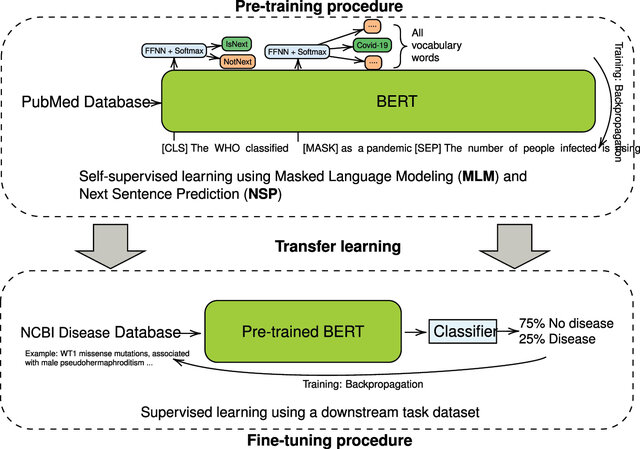
\includegraphics[width=0.78\textwidth]{../assets/figures/ch09-board-emb-img04.png}}
  \caption{فرایند پیش‌آموزش و انتقال یادگیری برای \eng{BERT}: بالا، پیش‌آموزش خودنظارتی با \eng{MLM} و \eng{NSP} (دو سر خروجی روی مدل)؛ پایین، قرار دادن یک دسته‌بند روی \eng{BERT} پیش‌آموزش‌دیده و آموزش تکمیلی با داده برچسب‌دار \eng{Task} هدف. \textit{(برگرفته از تختهٔ کلاس)}}
  \label{fig:ch09-bert}
\end{figure}

\subsection{معماری و ابعاد}
\eng{BERT} یک شبکهٔ \eng{Transformer Encoder} است که به‌صورت دوطرفه روی دنبالهٔ ورودی کار می‌کند. نسخهٔ پایه (\eng{BERT-Base}) ۱۲ لایه، بردار پنهان ۷۶۸‌بعدی، ۱۲ سر توجه و حدود ۱۱۰ میلیون پارامتر دارد؛ نسخهٔ بزرگ (\eng{BERT-Large}) ۲۴ لایه، بُعد ۱۰۲۴ و حدود ۳۴۰ میلیون پارامتر. ورودی با توکن‌های ویژه ساخته می‌شود: \lr{[CLS]} در ابتدا، \lr{[SEP]} بین دو جمله و در انتها، و \lr{[MASK]} برای جای واژهٔ پوشانده‌شده. برای یک ورودی با مثلاً ۷۱ توکن، خروجی هر لایه ماتریسی $H\in\mathbb{R}^{71\times768}$ است: یک بردار ۷۶۸‌بعدی برای هر توکن.

برای پیش‌بینی واژهٔ ماسک‌شده، روی خروجی لایهٔ ۱۲ یک لایهٔ خروجی قرار می‌گیرد (روی تخته: «یک لایه خطی روی لایه ۱۲ گذاشته می‌شود»). ابعاد آن روی تخته چنین نوشته شده بود (شکل زیر): بردار $1\times768$ در موقعیت ماسک، با یک لایهٔ خطی $768\times768$ به بردار پنهان $1\times768$ و سپس با لایهٔ $768\times V$ به لاجیت‌هایی به‌طول \mbox{$V=30522$} می‌رسد. \eng{Softmax} روی این لاجیت‌ها احتمال هر واژهٔ فرهنگ را می‌دهد.

\begin{figure}[htbp]
\centering
\resizebox{0.95\textwidth}{!}{$
H_{\text{\lr{mask}}}\in\mathbb{R}^{1\times768}
\xrightarrow{\;\text{\lr{Linear: 768$\times$768}}\;}
\text{\lr{Hidden}}\in\mathbb{R}^{1\times768}
\xrightarrow{\;\text{\lr{Linear: 768$\times$30522}}\;}
\text{\lr{Logits}}\in\mathbb{R}^{1\times30522}
$}
\caption{ابعاد سر \eng{MLM} در \eng{BERT}: بردار موقعیت ماسک با دو لایهٔ خطی به لاجیت‌هایی به‌طول اندازهٔ واژگان تبدیل می‌شود. (بازسازی‌شده از تختهٔ کلاس)}
\end{figure}

\begin{correctionbox}{جزئیات دقیق \eng{BERT} و وضعیت \eng{NSP}}
\begin{itemize}
  \item در \eng{MLM} حدود ۱۵ درصد توکن‌های ورودی برای پیش‌بینی انتخاب می‌شوند. از این توکن‌های انتخاب‌شده، ۸۰ درصد با \lr{[MASK]} جایگزین می‌شوند، ۱۰ درصد با یک توکن تصادفی و ۱۰ درصد بدون تغییر می‌مانند. دلیل این ترکیب آن است که \lr{[MASK]} در زمان استفاده هرگز وجود ندارد و مدل نباید فقط بر آن تکیه کند. خطا فقط روی همین توکن‌های انتخاب‌شده حساب می‌شود.
  \item در \eng{NSP}، نیمی از نمونه‌ها ادامهٔ واقعی (\eng{IsNext}) و نیم دیگر جملهٔ تصادفی (\eng{NotNext}) هستند. بعدها پژوهش‌هایی مانند \eng{RoBERTa} نشان دادند که حذف \eng{NSP} آسیبی نمی‌زند (و حتی مفید است)؛ بنابراین \eng{NSP} بخش ضروری ایدهٔ پیش‌آموزش نیست، هرچند در توضیح \eng{BERT} اصلی جزو آن بود.
  \item عدد $30522$ اندازهٔ واژگان \eng{WordPiece} در \eng{bert-base-uncased} (انگلیسی) است. مدل‌های فارسی یا چندزبانه واژگان متفاوتی دارند، پس $V$ به مدل بستگی دارد. توکن‌ها زیرواژه‌اند و همیشه با واژه برابر نیستند.
  \item دو خروجی \eng{MLM} و \eng{NSP} فقط برای پیش‌آموزش‌اند و هنگام استفاده معمولاً کنار گذاشته می‌شوند.
\end{itemize}
\end{correctionbox}

\subsection{استفاده از \eng{BERT}: استخراج بردار و انتقال یادگیری}
پس از پیش‌آموزش، سر \eng{MLM} دیگر به کار ما نمی‌آید و حذف می‌شود؛ وزن‌های لایه‌های ۱ تا ۱۲ نگه داشته می‌شوند. دو شیوهٔ استفاده روی تخته آمده بود:
\begin{enumerate}
  \item \textbf{استخراج بردار}: یک جمله به شبکه می‌دهیم؛ خروجی لایهٔ ۱۲ برای هر واژه یک بردار ۷۶۸ عددی اعشاری است. با برداشتن اندیس واژهٔ موردنظر، \eng{Embedding} بافتی آن واژه به دست می‌آید؛ و با میانگین‌گیری روی همهٔ واژه‌ها، یک \eng{Embedding} برای کل جمله ساخته می‌شود.
  \item \textbf{انتقال یادگیری}\ (\eng{Transfer Learning}): روی کل شبکه یک دسته‌بند می‌گذاریم و با داده‌ای محدود و مرتبط با \eng{Task} خود، همان لایه (و در صورت نیاز کل شبکه) را آموزش می‌دهیم (\eng{Fine-tuning}).
\end{enumerate}

\begin{addedbox}{نکته دربارهٔ بردار جمله}
میانگین‌گیری بردارهای توکن‌ها روشی ساده و رایج برای ساخت بردار جمله است، اما بردار \lr{[CLS]} یا میانگین لایه‌های مختلف هم گاهی استفاده می‌شود و کیفیت هر روش به \eng{Task} بستگی دارد. مدل‌هایی که مخصوصاً برای بردار جمله آموزش دیده‌اند معمولاً برای مقایسهٔ شباهت جمله‌ها از میانگین خام \eng{BERT} بهترند.
\end{addedbox}

\begin{exambox}{پرسش: آیا افزودن لایهٔ بیشتر (\eng{Linear} یا \eng{MLP}) همیشه بهتر است؟}
نمی‌توان قطعی گفت که افزودن یک لایه یا \eng{MLP} به‌طور حتم عملکرد را بهتر یا بدتر می‌کند. اگر یک لایهٔ ساده مسئله را حل می‌کند، دلیلی برای پیچیده‌تر کردن نیست؛ اگر عملکرد خوب نیست، شاید لازم باشد ظرفیت بخش دسته‌بند بیشتر شود. تصمیم باید بر اساس خطای آموزش، خطای اعتبارسنجی و وضعیت بایاس/واریانس گرفته شود. در همین زمینه به نسخه‌های مختلف \eng{BERT} (پایه و بزرگ) هم اشاره شد.
\end{exambox}

\section{قیاس برداری (\eng{Analogy}) در فضای \eng{Embedding}}

اگر روابط معنایی یا ساختاری به‌خوبی در فضای \eng{Embedding} بازتاب یافته باشند، اختلاف بردارهای دو جفت واژهٔ هم‌رابطه ممکن است تقریباً یکسان باشد. مثال مشهور:
\[
\vec{v}_{\text{\lr{king}}}-\vec{v}_{\text{\lr{man}}}+\vec{v}_{\text{\lr{woman}}}\approx\vec{v}_{\text{\lr{queen}}}
\quad\Longleftrightarrow\quad
\vec{v}_{\text{\lr{woman}}}-\vec{v}_{\text{\lr{man}}}\approx\vec{v}_{\text{\lr{queen}}}-\vec{v}_{\text{\lr{king}}} .
\]
یعنی «جهت» مفهوم «زن‌بودن در برابر مرد‌بودن» در دو جفت یکی است. استاد توضیح داد که چنین الگوهایی نشانهٔ سازمان‌یافتگی مفید فضای \eng{Embedding} هستند، اما برای همهٔ واژه‌ها و همهٔ مدل‌ها تضمین‌شده نیستند.

\coursefigure{0.55}{ch09-analogy-2d.png}{نمودار دوبعدی ساختگی برای قیاس برداری: بردار «زن $-$ مرد» (پیکان پیوسته) تقریباً با «ملکه $-$ شاه» (پیکان خط‌چین) موازی است و $\text{\lr{king}}-\text{\lr{man}}+\text{\lr{woman}}$ نزدیک نقطهٔ ملکه می‌افتد. محورها در فضای واقعی تفسیر ساده ندارند. (شکل افزوده)}

\begin{addedbox}{مثال عددی: قیاس برداری با شباهت کسینوسی}
فرض کنید در یک فضای دوبعدی ساختگی مختصات واژه‌ها به این صورت باشد: \mbox{$\text{\lr{man}}=(0.2,-0.9)$}، \mbox{$\text{\lr{woman}}=(0.1,1.0)$}، \mbox{$\text{\lr{king}}=(1.0,-1.1)$}، \mbox{$\text{\lr{queen}}=(0.95,0.85)$}، \mbox{$\text{\lr{prince}}=(0.6,-0.7)$}، \mbox{$\text{\lr{princess}}=(0.55,0.8)$} و \mbox{$\text{\lr{girl}}=(-0.1,0.7)$}. بردار هدف:
\[
t=\text{\lr{king}}-\text{\lr{man}}+\text{\lr{woman}}=(1.0-0.2+0.1,\;-1.1+0.9+1.0)=(0.9,\,0.8).
\]
شباهت کسینوسی \mbox{$\cos(a,b)=\dfrac{a\cdot b}{\|a\|\,\|b\|}$} را برای ملکه حساب می‌کنیم: \mbox{$a\cdot b=0.9\times0.95+0.8\times0.85=1.535$}، \mbox{$\|t\|=1.204$}، \mbox{$\|\text{\lr{queen}}\|=1.275$}، پس \mbox{$\cos\approx 1.535/(1.204\times1.275)\approx 0.9999$}. برای بقیه:
\begin{center}
\small
\begin{tabular}{lcccccc}
\toprule
واژه & \eng{queen} & \eng{princess} & \eng{woman} & \eng{girl} & \eng{prince} & \eng{man}\\
\midrule
\mbox{$\cos(t,\cdot)$} & $1.000$ & $0.971$ & $0.735$ & $0.552$ & $-0.018$ & $-0.486$\\
\bottomrule
\end{tabular}
\end{center}
نزدیک‌ترین واژه به $t$ ملکه است. توجه کنید که در آزمون‌های واقعی واژه‌های ورودی (\eng{king}، \eng{man}، \eng{woman}) از فهرست پاسخ‌ها کنار گذاشته می‌شوند؛ وگرنه معمولاً خود یکی از آن‌ها (مثلاً \eng{king}) نزدیک‌ترین است.
\end{addedbox}

\subsection{قیاس در \eng{Embedding} واج‌ها}
همین ایده در گفتار هم مطرح است. استاد به مقاله‌ای با عنوان «\lr{[b] = [d] − [t] + [p]}: مدل‌های گفتاری خودنظارتی حساب برداری واجی را کشف می‌کنند» (چوی و همکاران) اشاره کرد. بر اساس چکیدهٔ آن مقاله، در فضای بازنمایی مدل‌های گفتاری خودنظارتی \emph{جهت‌های خطی} متناظر با ویژگی‌های واجی وجود دارد؛ تفاضل $[d]-[t]$ یک «بردار واک‌داری» (\eng{Voicing}) می‌دهد، افزودن آن به $[p]$ تقریباً $[b]$ را می‌دهد، و مقیاس‌کردن آن، پیوستاری از واک‌داری ایجاد می‌کند. مقاله گزارش می‌دهد که از این بردارها می‌توان برای کنترل سنتز گفتار هم استفاده کرد. روی تخته هم همین مثال آمده بود:
\[
\vec{v}_{[d]}-\vec{v}_{[t]}+\vec{v}_{[p]}\approx\vec{v}_{[b]},\qquad\text{یعنی}\qquad \vec{v}_{[d]}-\vec{v}_{[t]}\approx\vec{v}_{[b]}-\vec{v}_{[p]}.
\]
در هر دو جفت، تفاوت اصلی «واک‌داری» است؛ ویژگی‌هایی مانند جایگاه تولید (\eng{Place of Articulation}) و شیوهٔ تولید (\eng{Manner of Articulation}) نیز می‌توانند جهت‌های مشابهی داشته باشند.

\begin{figure}[htbp]
  \centering
  \fbox{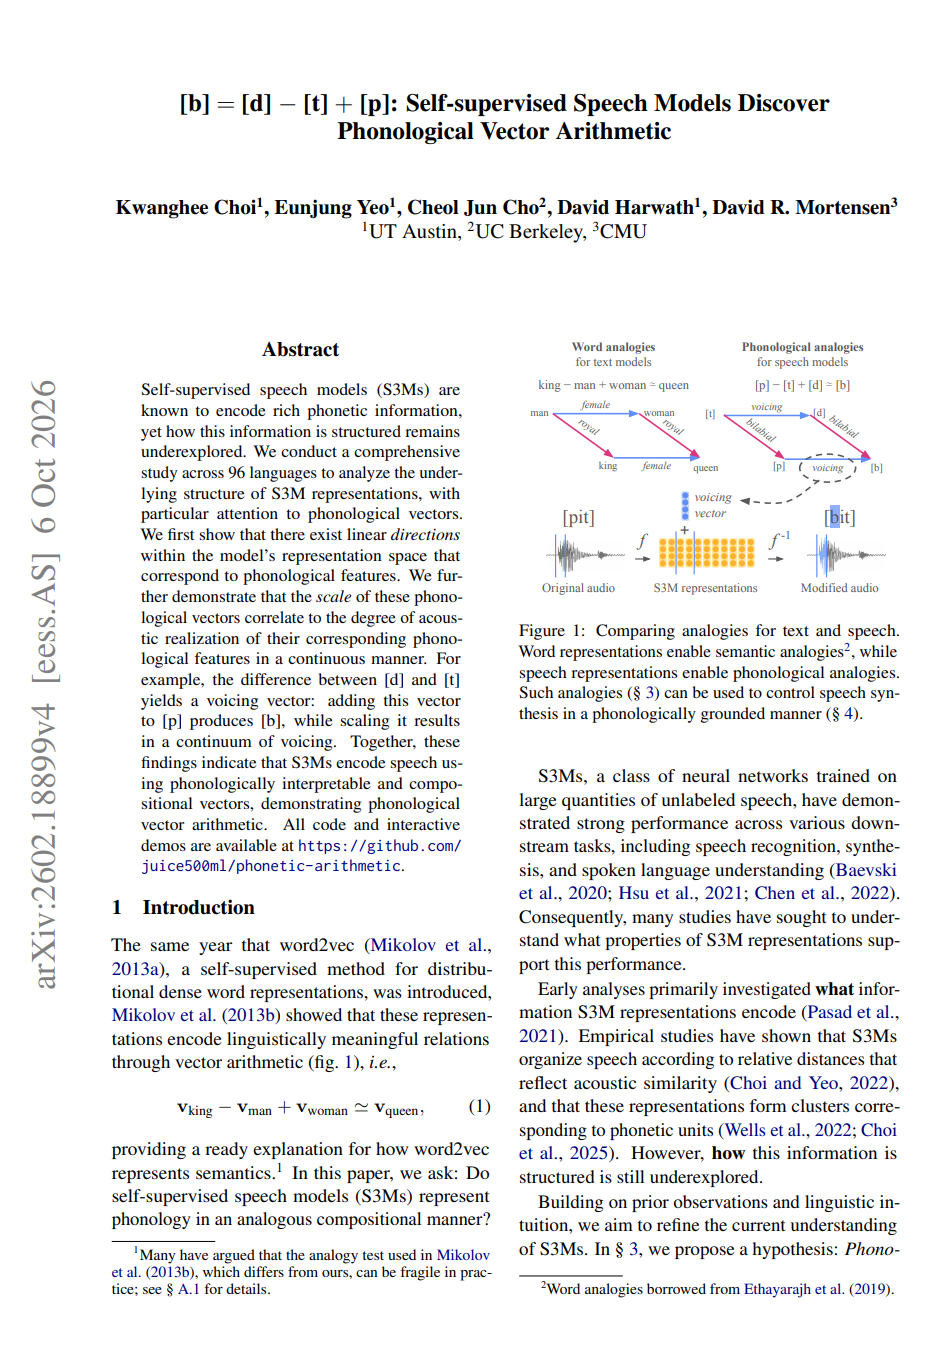
\includegraphics[width=0.62\textwidth]{../assets/figures/ch09-board-emb-img09.png}}
  \caption{صفحهٔ نخست مقالهٔ «\lr{[b] = [d] − [t] + [p]}». شکل ۱ مقاله قیاس واژه‌ای (\eng{king - man + woman}) را با قیاس واجی (\eng{[p] - [t] + [d] = [b]}) مقایسه می‌کند. \textit{(برگرفته از تختهٔ کلاس)}}
\end{figure}

\subsection{کاربردهای مطرح‌شده}
در بحث کلاس چند ایده مطرح شد: کشف ویژگی‌های آموخته‌شدهٔ مدل؛ کمک به پیش‌بینی در فضای \eng{Embedding}؛ سنجش دقت مدل (روی تخته: «میزان دقت مدل را فهمید»)؛ بررسی ویژگی‌های مرتبط با لهجه؛ و کاربرد احتمالی در سنتز گفتار و شبیه‌سازی صدا (\eng{Voice Cloning}). دربارهٔ لهجه، ایدهٔ استاد این بود که اگر بتوان برداری متناظر با یک ویژگی لهجه پیدا کرد، شاید بتوان آن را برای انتقال آن ویژگی در سنتز به کار برد. این در کلاس یک ایدهٔ قابل بررسی بود، نه نتیجه‌ای قطعی؛ و افزایش تفسیرپذیری بازنمایی‌ها از اهداف دیگر این رویکرد است.

\begin{correctionbox}{محدودیت‌های قیاس برداری}
قیاس‌هایی مانند \mbox{$\text{\lr{king}}-\text{\lr{man}}+\text{\lr{woman}}\approx\text{\lr{queen}}$} در مثال‌های خوب‌انتخاب‌شده و برای \eng{Embedding} ایستا (مانند \eng{Word2Vec}) به‌خوبی دیده می‌شوند، اما همیشه برقرار نیستند. بسیاری از روابط شکست می‌خورند، نتیجه به کنار گذاشتن واژه‌های ورودی از نامزدها وابسته است، و این روابط می‌توانند سوگیری‌های داده (مثلاً کلیشه‌های جنسیتی) را هم منعکس کنند. در \eng{Embedding} بافتی هم هر واژه یک بردار ثابت ندارد، بنابراین باید بازنمایی‌ها را به‌شکل مناسبی (مثلاً میانگین روی رخدادها) تعریف کرد. نتیجه: قیاس برداری یک ابزار تحلیل شهودی است، نه قانون.
\end{correctionbox}

\section{کاوش (\eng{Probing}) و تفسیرپذیری}
\label{sec:ch09-probing}

\subsection{\eng{Probing} چیست؟}
روی تخته پرسش‌های محوری چنین بود: «درون جعبهٔ سیاه یک شبکهٔ عصبی چه می‌گذرد؟ لایه‌های مختلف دقیقاً چه نوع اطلاعاتی را در خود ذخیره می‌کنند؟» استاد \eng{Probing} را به پروب‌زدن در مدار الکترونیکی تشبیه کرد: در نقاط مختلف مدار اندازه می‌گیریم تا ببینیم چه اتفاقی افتاده است.

\begin{definitionbox}{\term{دسته‌بند کاوشگر}{Probing Classifier}}
\eng{Probe} یک مدل کوچک و ساده (معمولاً یک لایهٔ خطی یا رگرسیون لجستیک) است که روی خروجی یک لایهٔ مشخص از یک شبکهٔ آموزش‌دیده و \emph{منجمد‌شده} آموزش داده می‌شود تا یک ویژگی زبانی یا گفتاری را پیش‌بینی کند. دقت این دسته‌بند معیار این است که آن اطلاعات در آن لایه تا چه حد «قابل استخراج» است.
\end{definitionbox}

\subsection{روش انجام}
\begin{enumerate}
  \item یک مدل پیش‌آموزش‌دیده را انتخاب و وزن‌هایش را فریز (ثابت) می‌کنیم.
  \item یک لایه (مثلاً یکی از لایه‌های میانی) را برای قرار دادن پروب انتخاب می‌کنیم؛ پرسش تخته‌ای: «کجا پراب بگذارم؟ لایه‌های میانی».
  \item نمایش‌های آن لایه را برای داده‌های برچسب‌دار استخراج می‌کنیم؛ مثلاً برای دنبالهٔ واج ورودی (\eng{Task: Phoneme Recognition})، دستهٔ \eng{Manner of Articulation} هر توکن که پروب باید با یک دسته‌بند در سطح توکن (\eng{Token Classification}) مشخص کند.
  \item یک دسته‌بند کوچک روی این نمایش‌ها آموزش می‌دهیم.
  \item دقت (\eng{Accuracy}) را روی داده‌ای کنار گذاشته‌شده می‌سنجیم.
\end{enumerate}
اگر پروب بتواند کلاس‌ها را با دقت خوبی تشخیص دهد، شاهدی داریم که آن اطلاعات در بازنمایی آن لایه وجود دارد. هدف اصلی از نگاه استاد این نیست که صرفاً بپرسیم ویژگی دقیقاً در کدام لایه آموخته شده، بلکه این است که آیا مدل اساساً آن اطلاعات را یاد گرفته یا نه. نمونه‌هایی که در کلاس بررسی شد: اطلاعات واجی، زبان، گوینده، و ویژگی‌هایی مانند شیوهٔ تولید (مثلاً تفکیک واکه‌ها و خیشومی‌ها).

\begin{figure}[htbp]
\centering
\begin{tikzpicture}[rtl, 
  layer/.style={draw,rounded corners=2pt,minimum width=3.6cm,minimum height=0.65cm,fill=gray!15,font=\small},
  probe/.style={draw,rounded corners=2pt,minimum width=2.4cm,minimum height=0.7cm,fill=orange!25,font=\small,align=center},
  ar/.style={-{Stealth[length=2mm]},thick}]
  \node[layer] (l0) {\lr{input}};
  \node[layer,above=0.35cm of l0] (l1) {\lr{layer 1}};
  \node[layer,above=0.35cm of l1] (l2) {\lr{layer 2}};
  \node[above=0.1cm of l2] (dots) {$\vdots$};
  \node[layer,above=0.45cm of dots] (l12) {\lr{layer 12}};
  \draw[ar] (l0)--(l1); \draw[ar] (l1)--(l2); \draw[ar] (l2)--(dots); \draw[ar] (dots)--(l12);
  \draw[dashed] ($(l0.south west)+(-0.25,-0.25)$) rectangle ($(l12.north east)+(0.25,0.25)$);
  \node[font=\small,below=0.35cm of l0] {مدل اصلی: وزن‌ها فریز};
  \node[probe,right=2cm of l2] (p) {دسته‌بند کوچک\\(پروب)};
  \node[right=0.8cm of p,font=\small,align=center] (o) {مثلاً دستهٔ\\\lr{Manner of Articulation}};
  \draw[ar] (l2.east)--(p.west) node[midway,above,font=\scriptsize]{نمایش لایه};
  \draw[ar] (p)--(o);
\end{tikzpicture}
\caption{ساختار \eng{Probing}: فقط پروب آموزش می‌بیند و مدل اصلی ثابت می‌ماند. (شکل افزوده)}
\end{figure}

\subsection{تفاوت \eng{Visualization} و \eng{Probing}}
برای نمایش \eng{Embedding}ها معمولاً از کاهش بُعد (مانند \eng{PCA} و \eng{t-SNE}) استفاده می‌شود. ممکن است در تصویر ببینیم دو کلاس از هم جدا شده‌اند، اما استاد تأکید کرد که این تصویر به‌تنهایی ثابت نمی‌کند مدل آن اطلاعات را به‌خوبی یاد گرفته است؛ برای شواهد دقیق‌تر باید یک \eng{Task} تعریف کرد و عملکرد آن را کمّی سنجید.

\begin{figure}[htbp]
  \centering
  \fbox{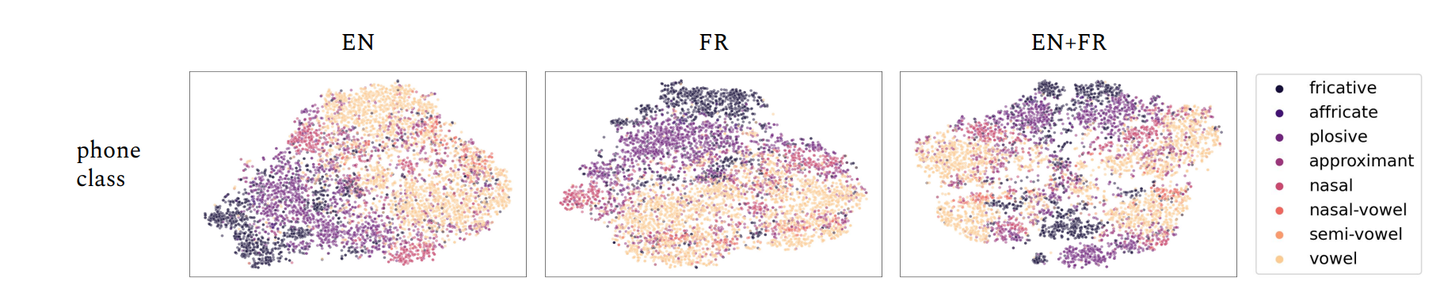
\includegraphics[width=0.95\textwidth]{../assets/figures/ch09-board-emb-img07.png}}
  \caption{نمایش \eng{t-SNE} بازنمایی‌های یک مدل گفتاری خودنظارتی برای سه مدل (آموزش‌دیده روی انگلیسی، فرانسوی و هر دو) با رنگ‌بندی بر اساس دستهٔ واج (سایشی، انسدادی، خیشومی، واکه و ...). خوشه‌های نسبتاً جدا دیده می‌شوند، اما این تصویر به‌تنهایی کمیت اطلاعات را اثبات نمی‌کند. \textit{(برگرفته از تختهٔ کلاس)}}
\end{figure}

\begin{table}[htbp]
\centering
\small
\begin{tabular}{p{3.2cm}p{5.5cm}p{5.5cm}}
\toprule
 & \textbf{\eng{Visualization}} & \textbf{\eng{Probing}}\\
\midrule
ماهیت & نمایش هندسی بردارها & ارزیابی اطلاعات قابل استخراج\\
روش & غالباً مبتنی بر کاهش بُعد & مبتنی بر یک \eng{Task} مشخص\\
نتیجه & عمدتاً بصری & معیار کمّی مانند \eng{Accuracy}\\
کاربرد & درک شهودی & ارائهٔ شواهد کمّی\\
\bottomrule
\end{tabular}
\caption{مقایسهٔ تجسم و کاوش.}
\end{table}

این مباحث در چارچوب \term{هوش مصنوعی توضیح‌پذیر}{Explainable AI} و \term{تفسیرپذیری}{Interpretability} قرار می‌گیرند: تلاش برای فهمیدن اینکه شبکه چه چیزهایی آموخته و چگونه از اطلاعات استفاده می‌کند.

\begin{correctionbox}{\eng{Probing} چه چیزی را ثابت می‌کند؟}
دقت بالای یک پروب نشان می‌دهد اطلاعات در نمایش \emph{وجود دارد و قابل استخراج است}، اما ثابت نمی‌کند خود مدل از آن برای حل \eng{Task} اصلی \emph{استفاده می‌کند}. همچنین اگر پروب بسیار پیچیده باشد، ممکن است خودش \eng{Task} را یاد بگیرد و نتیجه دربارهٔ نمایش چیزی نگوید؛ به همین دلیل پروب‌ها را ساده (مثلاً خطی) می‌گیرند و دقت را با یک مبنا (مثلاً مدل با وزن‌های تصادفی یا یک \eng{Control Task}) مقایسه می‌کنند. در \eng{t-SNE} نیز فاصله‌ها و اندازهٔ خوشه‌ها همیشه معنای دقیق ندارند و نتیجه به ابرپارامترها حساس است.
\end{correctionbox}

\section{بازگشت به \eng{TTS}: تلفظ درست هر واژه}

\subsection{جایگاه مسئله در خط لولهٔ \eng{TTS}}
در بخش پیشین دیدیم که \eng{Front-End} در \eng{TTS} پس از \term{نرمال‌سازی متن}{Text Normalization} باید تلفظ را مشخص کند. این کار با \term{تبدیل نویسه به واج}{Grapheme-to-Phoneme, G2P} انجام می‌شود. در فارسی، چون بسیاری از حرکات کوتاه نوشته نمی‌شوند، دو دشواری اصلی داریم: \term{هم‌نویسه‌ها}{Homograph} (یک شکل نوشتاری با تلفظ‌های متفاوت) و \term{واژه‌های خارج از واژگان}{Out-of-Vocabulary, OOV} (واژه‌ای که در فرهنگ تلفظ نیست).

\begin{table}[htbp]
\centering
\small
\begin{tabular}{p{2.0cm}p{4.2cm}p{4.2cm}p{3.2cm}}
\toprule
\textbf{نوشتار} & \textbf{تلفظ و معنی ۱} & \textbf{تلفظ و معنی ۲} & \textbf{ابزار تفکیک}\\
\midrule
مرد & \lr{/mæɾd/} «انسان مذکر» (اسم) & \lr{/moɾd/} «درگذشت» (فعل) & نقش دستوری (\eng{POS})\\
کرم & \lr{/keɾm/} «جانور خاکی»؛ \lr{/keɾem/} «ماده مرطوب‌کننده» & \lr{/kæɾæm/} «بخشندگی» (مثال افزوده) & معنای بافتی\\
گرم & \lr{/gæɾm/} «داغ» & \lr{/geɾæm/} «واحد جرم» & معنای بافتی\\
\bottomrule
\end{tabular}
\caption{نمونه‌هایی از هم‌نویسه‌های فارسی (بر اساس مثال‌های کلاس و تخته؛ نمادهای \eng{IPA} به‌صورت تقریبی‌اند).}
\end{table}

روی تخته توضیح داده شده بود که بسیاری از هم‌نویسه‌ها با تشخیص نقش دستوری یا معنای واژه در بافت قابل تفکیک‌اند: در «او مُرد» (فعل) و «آن مَرد رفت» (اسم) یک برچسب‌زن \eng{POS} (مثلاً \eng{hazm}) با تکیه بر دستور جمله کافی است. اما برای دو واژهٔ هم‌نقش، مانند «کِرم» خاکی و «کِرِم» مرطوب‌کننده که هر دو اسم‌اند، برچسب دستوری کمکی نمی‌کند و به بازنمایی بافت معنایی، یعنی \eng{Embedding} بافتی، نیاز داریم.

\subsection{طرح مهندسی: از ارزان به گران}
استاد مسیر زیر را پیشنهاد کرد (شکل~\ref{fig:ch09-flow}): پس از نرمال‌سازی، بررسی کنیم واژه در فرهنگ تلفظ هست یا نه. اگر هست و فقط یک تلفظ دارد، جست‌وجوی مستقیم؛ اگر چند تلفظ دارد، یک دسته‌بند بافتی؛ و اگر نیست (\eng{OOV})، واژه را به نویسه‌هایش بشکنیم و با یک مدل \eng{G2P} از نوع \eng{Sequence-to-Sequence} تلفظ را پیش‌بینی کنیم.

\begin{figure}[htbp]
\centering
\begin{tikzpicture}[rtl, 
  node distance=0.7cm and 0.5cm,
  box/.style={draw,rounded corners=2pt,minimum height=0.8cm,align=center,fill=blue!6,font=\small,inner sep=4pt},
  dec/.style={draw,diamond,aspect=2.2,align=center,fill=yellow!15,font=\small,inner sep=1pt},
  ar/.style={-{Stealth[length=2mm]},thick}]
  \node[box] (w) {واژه پس از نرمال‌سازی متن};
  \node[dec,below=0.6cm of w] (d1) {در فرهنگ\\هست؟};
  \node[dec,below left=1cm and 0.5cm of d1] (d2) {چند تلفظ\\دارد؟};
  \node[box,below right=1.1cm and 0.8cm of d1] (g2p) {مدل \lr{G2P}\\\lr{Seq2Seq}};
  \node[box,below left=1cm and 0.1cm of d2] (cls) {دسته‌بند بافتی\\\lr{Global Classifier}};
  \node[box,below right=1cm and 0.1cm of d2] (lk) {جست‌وجوی مستقیم\\در فرهنگ};
  \draw[ar] (w)--(d1);
  \draw[ar] (d1)-|node[pos=0.25,above,font=\scriptsize]{بله}(d2);
  \draw[ar] (d1)-|node[pos=0.25,above,font=\scriptsize]{خیر: \lr{OOV}}(g2p);
  \draw[ar] (d2)-|node[pos=0.25,above,font=\scriptsize]{بله}(cls);
  \draw[ar] (d2)-|node[pos=0.25,above,font=\scriptsize]{خیر}(lk);
\end{tikzpicture}
\caption{طرح تصمیم برای یافتن تلفظ: تا جای ممکن از روش‌های ارزان‌تر استفاده می‌شود. (شکل افزوده)}
\label{fig:ch09-flow}
\end{figure}

\subsection{رفع ابهام هم‌نویسه با دسته‌بندی}
اگر واژه فقط یک تلفظ ثبت‌شده دارد، همان را برمی‌داریم. اگر چند تلفظ دارد، باید یکی را متناسب با جمله انتخاب کنیم؛ این یک مسئلهٔ دسته‌بندی است، و اگر بیش از دو تلفظ ممکن باشد دسته‌بندی چندکلاسه. ورودی دسته‌بند همان \eng{Embedding} بافتی واژه است: جمله را وارد یک مدل \eng{Embedding} (مثلاً \eng{BERT}) می‌کنیم و بردار خروجی در موقعیت واژهٔ مبهم را به دسته‌بند می‌دهیم.

\subsubsection{چرا یک دسته‌بند سراسری؟}
پرسش کلاسی: چرا برای هر هم‌نویسه (مثلاً از ۵۰۰ هم‌نویسه) یک دسته‌بند جدا نسازیم؟ استاد دو دلیل برای \term{دسته‌بند سراسری}{Global Classifier} آورد:
\begin{enumerate}
  \item \textbf{اشتراک ویژگی‌ها}: نشانه‌های لازم برای تشخیص تلفظ میان واژه‌ها مشترک است؛ مثلاً قواعد نحوی، ساختاری و معنایی زبان. روی تخته نمونه‌قاعده این بود: «اگر قبل از کلمه حرف تعریف، ضمیر ملکی یا صفت آمد، یا کلمه در جایگاه فاعل یا مفعول نشست، این کلمه اسم است؛ پس کاندیدایی را فعال کن که برچسب اسمی دارد.» یک مدل مشترک می‌تواند چنین ویژگی‌هایی را یک بار یاد بگیرد و برای چند هم‌نویسه به کار ببرد.
  \item \textbf{کمبود داده}: برخی هم‌نویسه‌ها نمونهٔ فراوان دارند و برخی کم. دسته‌بند جداگانه روی واژه‌های کم‌تکرار یا بیش‌برازش می‌شود یا اصلاً یاد نمی‌گیرد. با وزن‌های مشترک (\eng{Shared Weights})، دانش از واژه‌های پرتکرار به واژه‌های کم‌تکرار منتقل می‌شود (\eng{Cross-word Transfer Learning}).
\end{enumerate}

\subsubsection{دسته‌بند شرطی (ماسک‌کردن کلاس‌های نامعتبر)}
اگر دسته‌بند سراسری روی مجموعهٔ بزرگی از تلفظ‌ها لاجیت می‌دهد، باید مطمئن شویم فقط تلفظ‌های معتبرِ همان واژه انتخاب می‌شوند. راه‌حل: پیش از \eng{Softmax}، لاجیت تلفظ‌های نامعتبر را برابر $-\infty$ می‌گذاریم:
\[
z_i'=\begin{cases} z_i & \text{اگر تلفظ } i \text{ برای این واژه معتبر باشد},\\ -\infty & \text{در غیر این صورت,}\end{cases}
\qquad P_i=\operatorname{Softmax}(z')_i .
\]
روی تخته هم برای واژهٔ «گرم» (کلاس‌های «\eng{garm}» و «\eng{geram}») نوشته شده بود: «گرفتن بیشینه فقط روی واج‌های مرتبط» (\eng{Getting maximum over only associated phonemes}).

\begin{addedbox}{مثال عددی: ماسک‌کردن کلاس‌ها}
فرض کنید برای واژهٔ «گرم» لاجیت‌ها چنین باشند: \eng{garm}:~$2.0$، \eng{geram}:~$0.5$ و تلفظ نامعتبر دیگری (مربوط به واژهٔ دیگر): $3.0$. بدون ماسک، \mbox{$e^{2}=7.389$}، \mbox{$e^{0.5}=1.649$} و \mbox{$e^{3}=20.086$} و مجموع $29.124$ است و احتمال‌ها \mbox{$(0.254,\,0.057,\,0.690)$} می‌شود؛ یعنی کلاس نامعتبر برنده است. با ماسک، فقط دو کلاس معتبر می‌مانند: مجموع $9.038$ و احتمال‌ها \mbox{$(0.818,\,0.182)$}؛ و \eng{garm} انتخاب می‌شود.
\end{addedbox}

\subsubsection{\eng{Greedy} یا \eng{Sampling}؟}
پرسش استاد (که کنار شکل روی تخته هم نوشته بود: «اینجا \eng{Argmax} یا تصادفی؟») پاسخ روشنی داشت: \eng{Greedy} یا \eng{Argmax}. در اینجا هدف انتخاب تلفظ درست است و برخلاف تولید متن خلاقانه به تنوع نیاز نداریم؛ پس پراحتمال‌ترین تلفظ معتبر انتخاب می‌شود.

\section{واژه‌های ناشناخته و \eng{G2P} از نوع \eng{Sequence-to-Sequence}}

\subsection{مسئله و داده}
برای واژه‌ای که در فرهنگ نیست نمی‌توان جست‌وجوی مستقیم کرد. ایده: واژه را به واحدهای کوچک‌تر، یعنی نویسه‌ها (\eng{Character}) بشکنیم و مدل، با تکیه بر الگوهایی که از دادهٔ آموزشی یاد گرفته، تلفظ را پیش‌بینی کند. داده‌های آموزشی را از خود فرهنگ تلفظ می‌سازیم: ورودی، دنبالهٔ نویسه‌های واژه و خروجی، دنبالهٔ واج‌های تلفظ درست:
\[
[g_1,g_2,\dots,g_n]\;\longrightarrow\;[p_1,p_2,\dots,p_m],\qquad n\neq m \text{ (در حالت کلی)}.
\]

نمونه‌هایی از این نابرابری طول را در فرهنگ تلفظ \eng{KaamelDict} (شکل~\ref{fig:ch07-kaameldict} در فصل هفتم) می‌توان دید؛ برای نمونه «شستشوهنده» و «واترپولو».

\begin{addedbox}{مثال: چرا \mbox{$n\neq m$}؟ (نمونه‌های فارسی)}
\begin{center}
\small
\begin{tabular}{p{1.6cm}p{2.6cm}p{0.8cm}p{2.5cm}p{0.8cm}p{3.6cm}}
\toprule
واژه & نویسه‌ها & $n$ & واج‌ها (\eng{IPA}) & $m$ & علت\\
\midrule
مدرسه & م، د، ر، س، ه & ۵ & \lr{m æ d ɾ e s e} & ۷ & حرکات کوتاه نوشته نمی‌شوند؛ «ه» پایانی \lr{/e/} است\\
خواب & خ، و، ا، ب & ۴ & \lr{x ɒ b} & ۳ & «و» پس از «خ» تلفظ نمی‌شود\\
مرد & م، ر، د & ۳ & \lr{m æ ɾ d} & ۴ & واکهٔ کوتاه \lr{/æ/} نوشته نمی‌شود\\
\bottomrule
\end{tabular}
\end{center}
پس نمی‌توان فرض کرد برای هر نویسه دقیقاً یک واج می‌آید. روی تخته هم نوشته شده بود که «در برخی زبان‌ها نگاشت یک به یک است» اما در فارسی استثنا، تشدید و سکون داریم.
\end{addedbox}

\subsection{چرا \eng{Seq2Seq}؟}
دسته‌بندی چندکلاسهٔ ساده یک ورودی را به یک برچسب از میان تعدادی کلاس ثابت می‌نگارد. اما در \eng{G2P} باید یک \emph{دنباله} تولید کنیم و طول آن به ورودی بستگی دارد و از پیش معلوم نیست. این مسئله از نوع \term{دنباله به دنباله}{Sequence-to-Sequence} است: دنبالهٔ ورودی $\leftarrow$ دنبالهٔ خروجی.

\subsection{معماری رمزگذار–رمزگشا}
\begin{itemize}
  \item \textbf{رمزگذار} (\eng{Encoder}): دنبالهٔ نویسه‌ها را می‌گیرد و نمایشی از ورودی می‌سازد که اطلاعات لازم برای تولید تلفظ را دارد (این مرحله، همان مفهوم \eng{Embedding} و درک دنباله است).
  \item \textbf{بردار زمینه} (\eng{Context Vector}): در توضیح تخته‌ای، آخرین حالت رمزگذار اطلاعات ورودی را خلاصه می‌کند و به رمزگشا می‌دهد. در معماری‌های دارای \eng{Attention}، رمزگشا به‌جای تکیه بر یک بردار ثابت به همهٔ حالت‌های خروجی رمزگذار دسترسی دارد.
  \item \textbf{رمزگشا} (\eng{Decoder}): دنبالهٔ واج‌ها را گام‌به‌گام تولید می‌کند. برای واج بعدی از اطلاعات رمزگذاری‌شدهٔ ورودی، واج‌های قبلاً تولیدشده و حالت فعلی خودش استفاده می‌کند.
\end{itemize}

\begin{figure}[htbp]
\centering
\begin{tikzpicture}[rtl, 
  tok/.style={draw,minimum width=0.85cm,minimum height=0.7cm,font=\small,fill=green!10},
  ph/.style={draw,minimum width=0.85cm,minimum height=0.7cm,font=\small,fill=orange!15},
  enc/.style={draw,rounded corners=3pt,minimum width=5.2cm,minimum height=0.9cm,fill=blue!10,font=\small},
  ar/.style={-{Stealth[length=2mm]},thick}]
  % graphemes (RTL reading kept as written order left-to-right for the toy figure)
  \foreach \i/\c in {1/م,2/د,3/ر,4/س,5/ه}{\node[tok] (g\i) at ({(6-\i)*0.95},0) {\c};}
  \node[enc] (E) at (2.85,1.5) {رمزگذار: \lr{Encoder}};
  \foreach \i in {1,...,5}{\draw[ar] (g\i)--(g\i |- E.south);}
  \node[enc,fill=orange!15,minimum width=5.8cm] (D) at (2.85,3.4) {رمزگشا: \lr{Decoder} + \lr{Cross-Attention}};
  \draw[ar] (E)--(D) node[midway,right,font=\scriptsize]{نمایش‌های ورودی};
  \foreach \i/\c in {1/m,2/æ,3/d,4/ɾ,5/e,6/s,7/e}{\node[ph] (p\i) at (\i*0.78-0.4,4.9) {\lr{\c}};}
  \foreach \i in {1,...,7}{\draw[ar] (D.north -| p\i)--(p\i);}
  \node[anchor=east,font=\small] at (0.3,0) {نویسه‌ها:};
  \node[anchor=east,font=\small] at (-0.05,4.9) {واج‌ها:};
\end{tikzpicture}
\caption{مدل \eng{G2P} با رمزگذار–رمزگشا برای واژهٔ «مدرسه» (۵ نویسه به ۷ واج). (شکل افزوده)}
\end{figure}

\subsection{\eng{Cross-Attention}}
در \eng{Self-Attention} یک دنباله برای ساخت نمایش خودش به عناصر همان دنباله توجه می‌کند. در \eng{Cross-Attention} یک دنباله (رمزگشا) به نمایش‌های دنبالهٔ دیگری (خروجی رمزگذار) توجه می‌کند. در \eng{G2P}، رمزگشا در حال تولید واج‌هاست؛ اطلاعات نویسه‌ها را رمزگذار آماده کرده است؛ و رمزگشا هنگام تولید واج بعدی می‌تواند به بخش‌های مرتبط ورودی توجه کند. تفاوت از نگاه کلاس: در \eng{Embedding} بافتی هدف ساخت نمایش یک عنصر با توجه به متن خودش بود، ولی در رمزگذار–رمزگشا رمزگشا برای ساخت خروجی به اطلاعات دنبالهٔ ورودی مراجعه می‌کند. در \eng{Cross-Attention} \eng{Query} از رمزگشا و \eng{Key} و \eng{Value} از خروجی رمزگذار می‌آیند.

\begin{addedbox}{آموزش در برابر استنتاج در رمزگشا}
در آموزش، به رمزگشا واج‌های درست قبلی داده می‌شود (روشی به نام \eng{Teacher Forcing}) و خطای \eng{Cross-Entropy} برای هر موقعیت خروجی جمع می‌شود. در استنتاج واج درست در دست نیست؛ رمزگشا باید واج‌هایی را که خودش تولید کرده در ورودی بعدی استفاده کند و تا تولید نشانهٔ پایان (\lr{<EOS>}) ادامه دهد. انتخاب هر واج در این مرحله معمولاً با \eng{Greedy} یا \eng{Beam Search} انجام می‌شود، نه نمونه‌گیری تصادفی، چون هدف یک تلفظ درست است.
\end{addedbox}

\subsection{مسائل دیگر از نوع \eng{Seq2Seq}}
این معماری فقط برای \eng{G2P} نیست؛ دو مثال مطرح‌شده: \term{ترجمهٔ ماشینی}{Machine Translation} (دنبالهٔ زبان مبدأ به دنبالهٔ زبان مقصد با طول احتمالاً متفاوت) و \term{خلاصه‌سازی انتزاعی}{Abstractive Summarization} (متن ورودی به یک خلاصهٔ تازه). در هر دو، خروجی دنباله است و طولش از پیش معلوم نیست.

\subsection{سطح بایت: مدل \eng{ByT5}}
روی تخته برای \eng{OOV} به مدل \eng{ByT5} (رمزگذار–رمزگشا) اشاره شده بود: مدلی که متن را در سطح بایت‌های \eng{UTF-8} (نویسه‌به‌نویسه) می‌خواند و بنابراین ورودی‌اش به واژه‌های از پیش‌معلوم وابسته نیست. موجودیت واژه در سطح کلمه شکسته می‌شود و توان تعمیم به واژه‌های دیده‌نشده پیدا می‌کند؛ انتظار این است که قواعد پنهان آوایی زبان را یاد بگیرد (مثلاً الگوی \lr{tion} را حتی اگر بخشی از واژه ناشناخته بود، «شن» بخواند).

\begin{addedbox}{ورودی بایتی برای فارسی}
در رمزگذاری \eng{UTF-8} هر نویسهٔ فارسی-عربی (مثل «م» یا «ه») دو بایت می‌گیرد و نیم‌فاصله (\eng{ZWNJ}) سه بایت. پس واژهٔ پنج‌نویسه‌ای «مدرسه» ۱۰ بایت است و ورودی \eng{ByT5} برای آن ۱۰ توکن بایتی خواهد بود؛ دنبالهٔ ورودی نسبت به مدل نویسه‌ای طولانی‌تر می‌شود. \eng{ByT5} را می‌توان بر روی جفت‌های (نویسه، واج) فرهنگ تلفظ تنظیم دقیق کرد.
\end{addedbox}

\section{ملاحظات مهندسی \eng{G2P} و بحث پایانی}

\subsection{چرا از ابتدا همه چیز را با \eng{Seq2Seq} حل نمی‌کنیم؟}
پرسش دانشجو: اگر \eng{G2P} دنباله‌به‌دنباله می‌تواند تلفظ همهٔ واژه‌ها را پیش‌بینی کند، چرا اصلاً سراغ فرهنگ و دسته‌بند برویم؟ پاسخ استاد: این یک تصمیم مهندسی است؛ روش‌ها از نظر هزینهٔ محاسباتی، نیاز به داده و پیچیدگی تفاوت دارند. ترتیب پیشنهادی:
\begin{enumerate}
  \item فرهنگ تلفظ برای واژه‌هایی که تلفظ مشخص دارند (بسیار کم‌هزینه).
  \item دسته‌بند برای هم‌نویسه‌ها.
  \item مدل \eng{G2P} دنباله‌به‌دنباله برای واژه‌های \eng{OOV} (آموزش و محاسبات بیشتر).
\end{enumerate}
استاد با یک شوخی دربارهٔ «اصفهانی‌بودن در مهندسی» تأکید کرد که باید از راه‌حل کم‌هزینه‌تر شروع کرد و فقط در صورت نیاز سراغ گزینه‌های گران‌تر رفت.

\begin{exambox}{آیا همیشه باید از فرهنگ شروع کنیم؟}
خیر. این ترتیب یک قاعدهٔ مهندسی است، نه الزام. اگر برای پروژهٔ شما فرهنگ مناسبی وجود ندارد یا زبان ورودی پر از واژه‌های جدید، محاوره‌ای و ساختارهای ناشناخته است (مثلاً متن شبکه‌های اجتماعی)، استفادهٔ مستقیم از مدل \eng{G2P} می‌تواند منطقی باشد. انتخاب معماری به شرایط پروژه بستگی دارد.
\end{exambox}

\subsection{ذخیرهٔ خروجی مدل در فرهنگ}
پرسش پایانی: وقتی مدل \eng{G2P} برای یک واژهٔ \eng{OOV} تلفظی ساخت، آیا لازم است دفعهٔ بعد دوباره مدل را اجرا کنیم؟ راهکار پیشنهادی: نتیجه را ذخیره (\eng{Cache}) و در مراجعه‌های بعدی استفاده کنیم؛ این کار هزینهٔ استنتاج را کم می‌کند. اما مطرح شد که تلفظ برخی واژه‌ها به بافت وابسته است؛ ذخیرهٔ یک تلفظ ثابت برای همهٔ واژه‌ها همیشه مناسب نیست و اگر تلفظ با جمله تغییر کند، سیستم باید این وابستگی را در نظر بگیرد.

\begin{correctionbox}{ذخیرهٔ نتیجه به‌معنای آموزش مجدد نیست}
در مرحلهٔ آموزش، مدل \eng{G2P} با واژه‌هایی که تلفظ‌شان مشخص است آموزش می‌بیند؛ در استنتاج برای واژه‌های جدید تلفظ پیش‌بینی می‌کند. ذخیرهٔ خروجی در فرهنگ یا حافظهٔ نهان یک تصمیم مهندسی جداگانه است و به‌خودی‌خود به معنی آموزش مجدد یا به‌روزرسانی وزن‌های مدل نیست. همچنین تلفظ خودکار ذخیره‌شده ممکن است خطا داشته باشد و بهتر است پیش از افزودن دائمی به فرهنگ بازبینی شود (پیشنهاد افزوده).
\end{correctionbox}

\section{جمع‌بندی}

در این فصل ابتدا لایهٔ خروجی و تابع خطا را بر اساس نوع مسئله (رگرسیون، دودویی، چندکلاسه) مرور کردیم و دیدیم که آموزش و استنتاج رفتار متفاوتی دارند: در آموزش حقیقت مبنا داریم و خطا حساب می‌کنیم، و در استنتاج از توزیع احتمال با روش‌هایی مانند \eng{Greedy}، \eng{Top-k}، \eng{Top-p} و \eng{Temperature} خروجی می‌گیریم. سپس با مقایسهٔ خطای آموزش و اعتبارسنجی، کم‌برازش (بایاس بالا) و بیش‌برازش (واریانس بالا) را شناختیم و ابزارهایی مانند توقف زودهنگام و منظم‌سازی را دیدیم.

در بخش دوم، \eng{Embedding} ایستا (جدول جست‌وجو، یک بردار برای هر واژه) را با \eng{Embedding} بافتی (تابعی از کل جمله و مستلزم اجرای شبکه) مقایسه کردیم. راه‌های ساخت بافتی (\eng{Self-Attention} و \eng{RNN/LSTM}) نشان داد که بافتی‌بودن با \eng{Transformer} هم‌ارز نیست. با یادگیری خودنظارتی (\eng{MLM} و \eng{NSP}) \eng{BERT} آموزش داده می‌شود و بردارهای ۷۶۸‌بعدی آن برای \eng{Task}های دیگر به کار می‌رود. قیاس برداری و \eng{Probing} هم روش‌هایی برای فهم اطلاعاتی‌اند که در بازنمایی‌ها ذخیره شده است.

در بخش سوم، این ابزارها به \eng{TTS} بازگشتند: برای هر واژه ابتدا فرهنگ، برای هم‌نویسه‌ها یک دسته‌بند سراسری با ماسک (و \eng{Argmax})، و برای واژه‌های ناشناخته یک مدل \eng{G2P} رمزگذار–رمزگشا با \eng{Cross-Attention}.

\begin{exambox}{نکات مهم برای مرور و امتحان}
\begin{enumerate}
  \item معماری و لایهٔ خروجی را بر اساس \eng{Task} طراحی کنید؛ لایه و نورون را بدون توجه به عملکرد زیاد نکنید.
  \item برای تشخیص مشکل مدل، خطای آموزش کافی نیست؛ خطای اعتبارسنجی و وضعیت بایاس/واریانس را هم ببینید.
  \item \eng{Contextual Embedding} را با \eng{Transformer} یکی نگیرید؛ مسئلهٔ اصلی ساخت نمایش وابسته به متن است و معماری‌های مختلفی (\eng{Attention}، \eng{LSTM}) برای آن وجود دارد.
  \item تفاوت ایستا (جدول جست‌وجو، فایل بردارها) و بافتی (وزن‌های شبکه، بردار فقط پس از دادن جمله) را بدانید.
  \item برای نشان‌دادن اینکه مدل چه اطلاعاتی یاد گرفته، فقط به \eng{Visualization} اکتفا نکنید؛ \eng{Probing} و معیارهای کمّی شواهد دقیق‌تری می‌دهند.
  \item در \eng{TTS}، هم‌نویسه‌ها و واژه‌های \eng{OOV} دو چالش متفاوت‌اند و با روش‌های متفاوت حل می‌شوند.
  \item دلایل استفاده از دسته‌بند سراسری برای هم‌نویسه‌ها: اشتراک ویژگی‌ها و کمبود داده؛ و در استنتاج کلاس‌های نامعتبر ماسک می‌شوند و \eng{Argmax} به کار می‌رود.
  \item \eng{G2P} برای \eng{OOV} از نوع \eng{Seq2Seq} است چون طول دنبالهٔ واج‌ها لزوماً برابر طول دنبالهٔ نویسه‌ها نیست.
  \item هزینهٔ محاسباتی مهم است: تا جای ممکن از فرهنگ و روش‌های ساده‌تر استفاده کنید و مدل‌های پیچیده را فقط وقتی لازم است وارد کنید.
\end{enumerate}
\end{exambox}

\begin{table}[htbp]
\centering
\small
\begin{tabular}{p{4.2cm}p{9.8cm}}
\toprule
\textbf{اصطلاح} & \textbf{مفهوم}\\
\midrule
\eng{Logit} & امتیاز خام پیش از تبدیل به احتمال\\
\eng{Softmax}, \eng{Sigmoid} & تبدیل لاجیت‌ها به توزیع احتمال (چندکلاسه) یا به عدد در $(0,1)$ (دودویی)\\
\eng{Greedy}, \eng{Sampling}, \eng{Top-k}, \eng{Top-p} & روش‌های انتخاب خروجی از توزیع احتمال در استنتاج\\
\eng{Temperature} & کنترل تیزی توزیع با تقسیم لاجیت‌ها بر $T$\\
\eng{Early Stopping} & توقف آموزش در کمینهٔ خطای اعتبارسنجی\\
\eng{Underfitting}, \eng{Overfitting} & ناتوانی در یادگیری الگوها، یا حفظ‌کردن نویز داده آموزش\\
\eng{Regularization} & محدودسازی پیچیدگی مؤثر مدل (\eng{Dropout}, \eng{L1}, \eng{L2})\\
\eng{Static}/\eng{Contextual Embedding} & بردار ثابت هر واژه / بردار وابسته به جمله\\
\eng{Self-Supervised Learning} & ساخت برچسب از خود داده\\
\eng{MLM}, \eng{NSP} & پیش‌بینی توکن ماسک‌شده؛ پیش‌بینی اینکه آیا جملهٔ دوم ادامهٔ جملهٔ اول است\\
\eng{Analogy} & قیاس برداری، مانند \mbox{$\text{\lr{king}}-\text{\lr{man}}+\text{\lr{woman}}\approx\text{\lr{queen}}$}\\
\eng{Probing} & آموزش دسته‌بند ساده روی خروجی لایه‌های فریزشدهٔ مدل برای سنجش اطلاعات قابل استخراج\\
\eng{Homograph}, \eng{OOV} & هم‌نویسه با تلفظ‌های متفاوت؛ واژهٔ خارج از فرهنگ\\
\eng{G2P}, \eng{Seq2Seq}, \eng{Encoder}/\eng{Decoder} & تبدیل نویسه به واج؛ نگاشت دنباله به دنباله؛ رمزگذار/رمزگشا\\
\eng{Cross-Attention} & توجه رمزگشا به نمایش‌های دنبالهٔ ورودی\\
\bottomrule
\end{tabular}
\caption{اصطلاحات کلیدی فصل.}
\end{table}
